% Use UTF-8 encoding!!
% (c) Stefan Ulbrich, 2012

\documentclass[english,ngerman]{KITreprt}


%% -------------------------------
%% |  Information for PDF file   |
%% -------------------------------
\hypersetup{
 pdfauthor={Patrick Niklaus},
 pdftitle={Bachelor Thesis: Walking pattern generation for humanoid bipedal robots},
 pdfsubject={Not set},
 pdfkeywords={Not set}
}


%% --------------------------------
%% Obligatory Parameters:
%% --------------------------------

\renewcommand{\myname}{Patrick Niklaus}
\renewcommand{\mythesis}{\bachelorsthesis} %\mastersthesis, \bachelorsthesis, \protocol, \studienarbeit, \diplomarbeit
\renewcommand{\mytitle}{ Dynamically Stable Walking For Humanoid Bipedal Robots Based On Walking Patterns }
%\renewcommand{\myshorttitle}{Die offizielle \LaTeX-Vorlage des HIS}
\renewcommand{\myshorttitle}{}
\cfoot{\mytitle}

\renewcommand{\timestart}{1. April 2014}
\renewcommand{\timeend}{1. Oktober 2014}
%\renewcommand{\timeend}{\iflanguage{english}{February 7\textsuperscript{th},}{7. Februar} 2010}
\newcommand{\advisor}{Dr. Júlia Borràs Sol}
%\newcommand{\advisortwo}{Nur wenn n\"otig}

\newcommand{\clr}[2]{{\color{#1}{#2}}}
%\newcommand{\todo}[1]{\marginpar{\clr{red}{#1}}}
%\newcommand{\todo}[1]{%
%    \addcontentsline{tdo}{todo}{\protect{#1}}
%    \marginpar{\clr{red}{#1}}
%}

% Command for inserting a todo item
\newcommand{\todo}[1]{%
% Add to todo list
\addcontentsline{tdo}{todo}{\protect{#1}}%
%
\begin{tikzpicture}[remember picture, baseline=-0.75ex]%
\node [coordinate] (inText) {};
\end{tikzpicture}%
%
% Make the margin par
\marginpar{%
\begin{tikzpicture}[remember picture]%
\definecolor{orange}{rgb}{1,0.5,0}
\draw node[draw=black, fill=orange, text width = 2.5cm] (inNote)
{#1};%
\end{tikzpicture}%
}%
%
\begin{tikzpicture}[remember picture, overlay]%
\draw[draw = orange, thick]
([yshift=-0.2cm] inText)
-| ([xshift=-0.2cm] inNote.west)
-| (inNote.west);
\end{tikzpicture}%
%
}% 

\newcommand{\slpy}[1]{{\sloppy #1}}
\newcommand{\fixme}[1]{{\color{red}{FIXME: #1}}}
\newcommand{\name}[1]{\textsc{#1}}
\makeatletter \newcommand \listoftodos{\section*{Todo list} \@starttoc{tdo}}
\newcommand\l@todo[2]
    {\par\noindent \textit{#2}, \parbox{10cm}{#1}\par} \makeatother

\graphicspath{{./images/}}


\begin{document}


\selectlanguage{english}

%\selectlanguage{ngerman}


\maketitle

\tableofcontents

\chapter{Introduction}\label{introduction}

motivation, and a bit of overview of humanoid walking. I recommend to
leave it for later, start with the sections that you feel its easier to
write (usually, the ones that have more content).

\begin{itemize}
\itemsep1pt\parskip0pt\parsep0pt
\item
  motivation:

  \begin{itemize}
  \itemsep1pt\parskip0pt\parsep0pt
  \item
    navigating in human environments
  \end{itemize}
\item
  walking in humans:

  \begin{itemize}
  \itemsep1pt\parskip0pt\parsep0pt
  \item
    CoM movement, gait phases, differences to what we do here
  \end{itemize}
\item
  static vs.~dynamic walking
\item
  overview of models used for dynamic walking
\end{itemize}

\chapter{Models for humanoid walking}\label{models-for-humanoid-walking}

\section{The Linear Inverted Pendulum
Model}\label{the-linear-inverted-pendulum-model}

\todo{Use different name for CoM, $p$ will be rather used for the ZMP, maybe $c$?}

\todo{picture of 3D-LIPM}

A simple model for describing the dynamics of a bipedal robot during
single support phase is the 3D inverted pendulum. We reduce the body of
the robot to a point-mass at the center of mass and replace the support
leg by a mass-less telescopic leg which is fixed at a point on the
supporting foot. Initially this will yield non-linear equations that
will be hard to control. Howevery by constraining the movement of the
inverted pendulum to a fixed plane, we can derive a linear dynamic
system. This model called the 3D \emph{linear} inverted pendulum model
(short \emph{3D-LIPM}).

\subsection{The inverted pendulum}\label{the-inverted-pendulum}

To describe the dynamics of the inverted pendulum we are mainly
interested in the effect a given actuator torque has on the movement of
the pendulum.

For simplicity we assume that the base of the pendulum is fixed at the
origin of the current cartesian coordinate system. Thus we can describe
the position inverted pendulum by a vector $p = (x, y, z)$. We are going
to introduce an appropriate (generalized) coordinate system
$q = (\theta_R, \theta_P, r)$ to get an easy description of our actuator
torques: Let $m$ be the mass of the pendulum and $r$ the length of the
telescopic leg. $\theta_P$ and $\theta_R$ describe the corresponding
roll and pitch angles of the pose of the pendulum.
\todo{add image with angles here}

Now we need to find a mapping between forces in the cartesian coordinate
system and the generalized forces (the actuator torques). Let
$\Phi: \mathbb{R}^3 \longrightarrow \mathbb{R}^3, (\theta_R, \theta_P, r) \mapsto (x, y, z)$
be a function that maps the generalized coordinates to the cartesian
coordinates. Then the jacobian $J_\Phi = \frac{\partial p}{\partial q}$
maps the \emph{generalized velocites} to \emph{cartesian velocites}.
Furthermore we know that the transpose $J_\Phi^T$ maps \emph{cartesian
forces} $F = m (\ddot x, \ddot y, \ddot z)$ to \emph{generalized forces}
$(\tau_r, \tau_p, f)$.

We write $x$, $y$ and $z$ in terms of our generalized coordinates to
compute the corresponding jacobian $J_\Phi$. From the fact that the
$\theta_P$ is the angle between the projection of $p$ onto the
$xz$-plane and $p$ and $\theta_R$ the angle between $p$ and the
projection onto the $yz$ plane we can derive the following equations
\todo{reference paper}:

\begin{equation}
\begin{array}{lcll} \label{eq:lip-xyz}
x & = & r \cdot \sin \theta_P & =: r \cdot s_P\\
y & = & -r \cdot \sin \theta_R & =: -r \cdot s_R \\
z & = & \sqrt{r^2 - x^2 - y^2} = r \cdot \sqrt{1 - s_P^2 - s_R^2} & \\
\end{array}
\end{equation}

From which we can compute the jacobian by partial derivation:

\begin{equation} \label{eq:lip-jacobian}
J = \frac{\partial p}{\partial q} = \left( \begin{array}{rcl}
0 & r \cdot c_P & s_P \\
-r \cdot c_R & 0 & s_P \\
\frac{2 \cdot r \cdot s_P c_P}{\sqrt{1 - s_P^2 - s_R^2}} & \frac{2 \cdot r \cdot s_R c_R}{\sqrt{1 - s_P^2 - s_R^2}} & \sqrt{1 - s_P^2 - s_R^2}\\
\end{array}
\right)
\end{equation}

Using the equation of motion as given by

\begin{equation}
\begin{array}{lcr}
F & = & (J^T)^{-1} \Gamma + f_g \\
m \cdot
\left(\begin{array}{c}
\ddot x \\
\ddot y \\
\ddot z \\
\end{array}\right)
& = & (J^T)^{-1}
\left(\begin{array}{c}
\tau_R \\
\tau_P \\
f \\
\end{array}\right)
+
\left(\begin{array}{c}
0 \\
0 \\
-m \cdot g \\
\end{array}\right) \\
\end{array}
\end{equation}

and equations \ref{eq:lip-jacobian} and \ref{eq:lip-xyz} we can derive
the following equations:

\begin{equation} \label{eq:lip-dyn-y}
m(-z\ddot{y} + y\ddot{z}) = \frac{\sqrt{1 - s_P^2 - s_R^2}}{c_R} \cdot \tau_R + m g y
\end{equation}

\begin{equation} \label{eq:lip-dyn-x}
m(z\ddot{x} - x\ddot{z}) = \frac{\sqrt{1 - s_P^2 - s_R^2}}{c_P} \cdot \tau_P + m g x
\end{equation}

Observe that the terms of the left-hand side are not linear. To remove
that non-linearity we are going to use the \emph{linear} inverted
pendulum model.

\subsection{Linearization}\label{linearization}

In a man-made environment it is fair to assume that the ground a robot
will walk on can be approximate by a slightly sloped plane. In most
cases it can even assumed that there is no slope at all.

The basic assumption in the next section will be that the CoM will have
a \emph{constant displacement} with regard to our ground plane. Thus we
can constrain the movement of the CoM to a plane that is parallel to the
ground plane. Note that this assumption is, depending on the walking
speed, only approximately true for human walking as shown by Orendurff
et. al. For slow to fast walking ($0.7$ m/s and $1.6$ m/s respectively)
the average displacement in $z$-direction was found to be between
$2.7cm$ and $4.81$ cm. While the walking patterns generated based on the
LIP-model will guarantee dynamic stability, they might not look natural
with regard to human walking.

\todo{cite Orendurff}

We are going to constrain the $z$ coordinate of our inverted pendulum to
a plane with normal vector $(k_x, k_y, -1)$ and $z$-displacement $z_c$:

\begin{equation} \label{eq:lip-z-plane}
z = k_x \cdot x + k_y \cdot y + z_c
\end{equation}

Subsequently the second derivative of $z$ can be described by:

\begin{equation} \label{eq:lip-z-div}
\ddot{z} = k_x \cdot \ddot{x} + k_y \cdot \ddot{y}
\end{equation}

Substituing \ref{eq:lip-z-plane} and \ref{eq:lip-z-div} into the
equations \ref{eq:lip-dyn-y} and \ref{eq:lip-dyn-x} yields the following
equations:

\begin{equation}
\ddot{y} = \frac{g}{z_c} y - \frac{k_x}{z_c} (x\ddot{y} - \ddot{x}y) - m z_c \cdot \tau_R \cdot \frac{\sqrt{1 - s_P^2 - s_R^2}}{c_R}
\end{equation}

\begin{equation}
\ddot{x} = \frac{g}{z_c} x + \frac{k_y}{z_c} (x\ddot{y} - \ddot{x}y) + m z_c \cdot \tau_P \cdot \frac{\sqrt{1 - s_P^2 - s_R^2}}{c_P}
\end{equation}

The term $x\ddot{y} - \ddot{x}y$ that is part of both equations is still
causing the equations to be non-linear. To make this equations linear we
will assume that our ground plane has no slope, thus $k_x = k_y = 0$ and
the non-linear terms will vanish.

Another problem is that the actuator torques $\tau_R$ and $\tau_P$ both
have non-linear factors $\frac{\sqrt{1 - s_P^2 - s_R^2}}{c_R}$ and
$\frac{\sqrt{1 - s_P^2 - s_R^2}}{c_P}$ respectively. This can be solved
by substituting with the following \emph{virtual inputs}:

\begin{equation}
\tau_P \cdot \frac{\sqrt{1 - s_P^2 - s_R^2}}{c_P} = u_P
\end{equation}

\begin{equation}
\tau_R \cdot \frac{\sqrt{1 - s_P^2 - s_R^2}}{c_R} = u_R
\end{equation}

Which yields our final description of the dynamics:

\begin{equation} \label{eq:lip-y}
\ddot{y} = \frac{g}{z_c} y - \frac{u_R}{m z_c}
\end{equation}

\begin{equation} \label{eq:lip-x}
\ddot{x} = \frac{g}{z_c} x + \frac{u_R}{m z_c}
\end{equation}

\todo{include pattern generation just based on 3D-LIPM, I don't understand how they derived the controller}

\section{The Zero Moment Point}\label{the-zero-moment-point}

A very popular approach to humanoid walking are schemes based on the
Zero Moment Point. One reason for that might be that it is very simple
to describe constrains for dynamic stability using this reference point.
As long as the following condition is met we will have full ground
contact of our support foot and thus can realize dynamically stable
walking: \emph{The ZMP is strictly inside the support polygone of the
support foot.}

For flat ground contact of our support foot with the floor the ZMP
corresponds with the position of the center of pressure (CoP). Indeed,
some author (notably Pratt) prefer to use the term CoP instead of ZMP.

The CoP of an object in contact with the ground can be computed as the
sum of all contact points $p_1, \dots, p_n$ weighted by the forces in
$z$-direction $f_{1z}, \dots, f_{nz}$ that is applied:

\begin{equation} \label{eq:zmp-definition}
p := \frac{\sum^N_{i=1}p_i f_{iz}}{\sum^N_{i=1} f_{iz}}
\end{equation}

An important fact (and the origin of its name) is that there are no
torques around the $x$ and $y$ axis at the ZMP:

\begin{equation}
\tau = \sum^N_{i=1} (p_i - p) \times f_i
\end{equation}

Splitting that up into each component using the definition of the cross
product yields:

\begin{equation}
\tau_x = \sum^N_{i=1} (p_{iy} - p_y) f_{iz} - \overbrace{(p_{iz} - p_z)}^{=0} f_{iy}
\end{equation}

\begin{equation}
\tau_y = \sum^N_{i=1} \overbrace{(p_{iz} - p_z)}^{=0} f_{ix} - (p_{ix} - p_x) f_{iz}
\end{equation}

\begin{equation}
\tau_z = \sum^N_{i=1} (p_{ix} - p_x) f_{iy} - (p_{iy} - p_y) f_{ix}
\end{equation}

Since we have flat ground contact, all contact points have the same
$z$-coordinate as the ZMP, thus we can simplify $\tau_x$ and $\tau_y$
to:

\begin{equation} \label{eq:zmp-torque-x}
\tau_x = \sum^N_{i=1} (p_{iy} - p_y) f_{iz} = \sum^N_{i=1} (p_{iy} f_{iz}) - (\sum^N_{i=0} f_{iz}) \cdot p_y
\end{equation}

\begin{equation}\label{eq:zmp-torque-y}
\tau_y = \sum^N_{i=1} - (p_{ix} - p_x) f_{iz} = \sum^N_{i=1} - (p_{ix} f_{iz}) + (\sum^N_{i=0} f_{iz}) \cdot p_x
\end{equation}

Furthermore we can use the corresponding components $p_x$ and $p_y$ from
the definition of the ZMP \ref{eq:zmp-definition} and substitude in the
equations \ref{eq:zmp-torque-x} and \ref{eq:zmp-torque-y}.

This will yield: $\tau_x = \tau_y = 0$.

Please note that $\tau_z$ will in general not be zero, nonetheless in
case of straight walking it is often assumed to be zero as well.

\section{The table-cart model}\label{section:table-cart}

The table-cart model is equivalent to the 3D-LIPM model discussed
before, but somewhat more intuitive for computing the resulting ZMP from
an CoM motion. The model consists of an (infinitely) large mass-less
table of height $z_c$, while the foot of the table has the shape of the
support polygone. Given a frictionless cart with mass $m$ that moves on
the table we can compute the resulting ZMP in the support foot. Please
note that the 3D-dimensional model is equivalent to having two
independent tables with two carts each in the $xz$ and $yz$-plane
respectively. First of all, lets compute the torque $\tau_x$ and
$\tau_y$ around the x-axis and y-axis at the ZMP on the support foot.

\begin{equation}
\tau_y = \overbrace{-m g (c_x - p_x)}^{\text{torque due to gravity}} + \overbrace{m \ddot{x} \cdot z_c}^{\text{torque due to acceleration of cart}}
\end{equation}

\begin{equation}
\tau_x = -m g (c_y - p_y) + m \ddot{y} \cdot z_c
\end{equation}

Please note the similarity to the equations \ref{eq:lip-y} and
\ref{eq:lip-x} when assuming the base of the pendulum is located at $p$.
If we now use the property of the ZMP that the torque around the $x$ and
$y$-axis is zero, we can solve for the ZMP position $p$:

\begin{equation} \label{eq:zmp-x}
p_x = c_x - \frac{z_c}{g} \ddot{c_x}
\end{equation}

\begin{equation} \label{eq:zmp-y}
p_y = c_y - \frac{z_c}{g} \ddot{c_y}
\end{equation}

\section{Multi-Body methode to calculate the
ZMP}\label{section:multi-body-zmp}

Besides the simplified table-cart model, there also exsists an exact
methode to calculate the resulting ZMP from the movement from serveral
connected rigid bodies.

Let $c_i$ be the CoM position and $m_i$ the mass of the $i$-th body
($i \in \{1, ..., k\}$). Then the total linear momentum $\mathcal{P}$
can be calculated by:

\begin{equation}
\mathcal{P} = \sum^k_{j=1} m_j \cdot \dot{c}_j
\end{equation}

If $\omega_i$ the angular momentum and $R_i$ is the rotational part of
the reference frame of the $i$-th body and $I_i$ the inertia tensor in
that reference frame, the total angular momentum $\mathcal{L}$ can be
calculated by:

\begin{equation}
\mathcal{L} = \sum^k_{j=1} c_j \times (m_j \dot{c}_j) + R_j I_j R^T_j \omega_j
\end{equation}

If we denote the total mass of the robot with $M$ and the gravity vector
with $g$ we can express the change of linear momentum if a force $f$ is
applied to the body as:

\begin{equation} \label{eq:change-lin-momentum}
\dot{\mathcal{P}} = M g + f
\end{equation}

And subsequently the change in angular momentum if a torque $\tau$ is
applied:

\begin{equation} \label{eq:change-ang-momentum}
\dot{\mathcal{L}} = c \times Mg + \tau
\end{equation}

To calculate the resulting torque $\tau_{ZMP}$ around the ZMP located at
$p$ we can use:

\begin{equation} \label{eq:multi-body-zmp}
\tau_{ZMP} = \tau + (0 - p) \times f = \tau - p \times f
\end{equation}

If solve equation \ref{eq:change-lin-momentum} for $f$ and
\ref{eq:change-ang-momentum} for $\tau$ and substitute them in
\ref{eq:multi-body-zmp} this yields the following equation:

\begin{equation}
\tau_{ZMP} = \dot{\mathcal{L}} - c \times M g - p \times (\dot{\mathcal{P}} - Mg)
\end{equation}

Since we know that the torque around the ZMP is zero around the $x$ and
$y$ axis we can apply the definition of the cross product and solve for
the ZMP position:

\begin{equation}
p_x = \frac{Mgx + p_z \dot{\mathcal{P}}_x - \dot{\mathcal{L}}_y}{Mg + \dot{\mathcal{P}}_z}
\end{equation}

\begin{equation}
p_y = \frac{Mgy + p_z \dot{\mathcal{P}}_y - \dot{\mathcal{L}}_x}{Mg + \dot{\mathcal{P}}_z}
\end{equation}

Both equations are dependent on $p_z$. If we assume the robot walks on a
flat floor, we can set $p_z = 0$.

See figure \ref{zmp-comparision} to get an idea how much the Multi-Body
ZMP derives from the estimation using the Cart-Table model.

\begin{figure*}[tb]
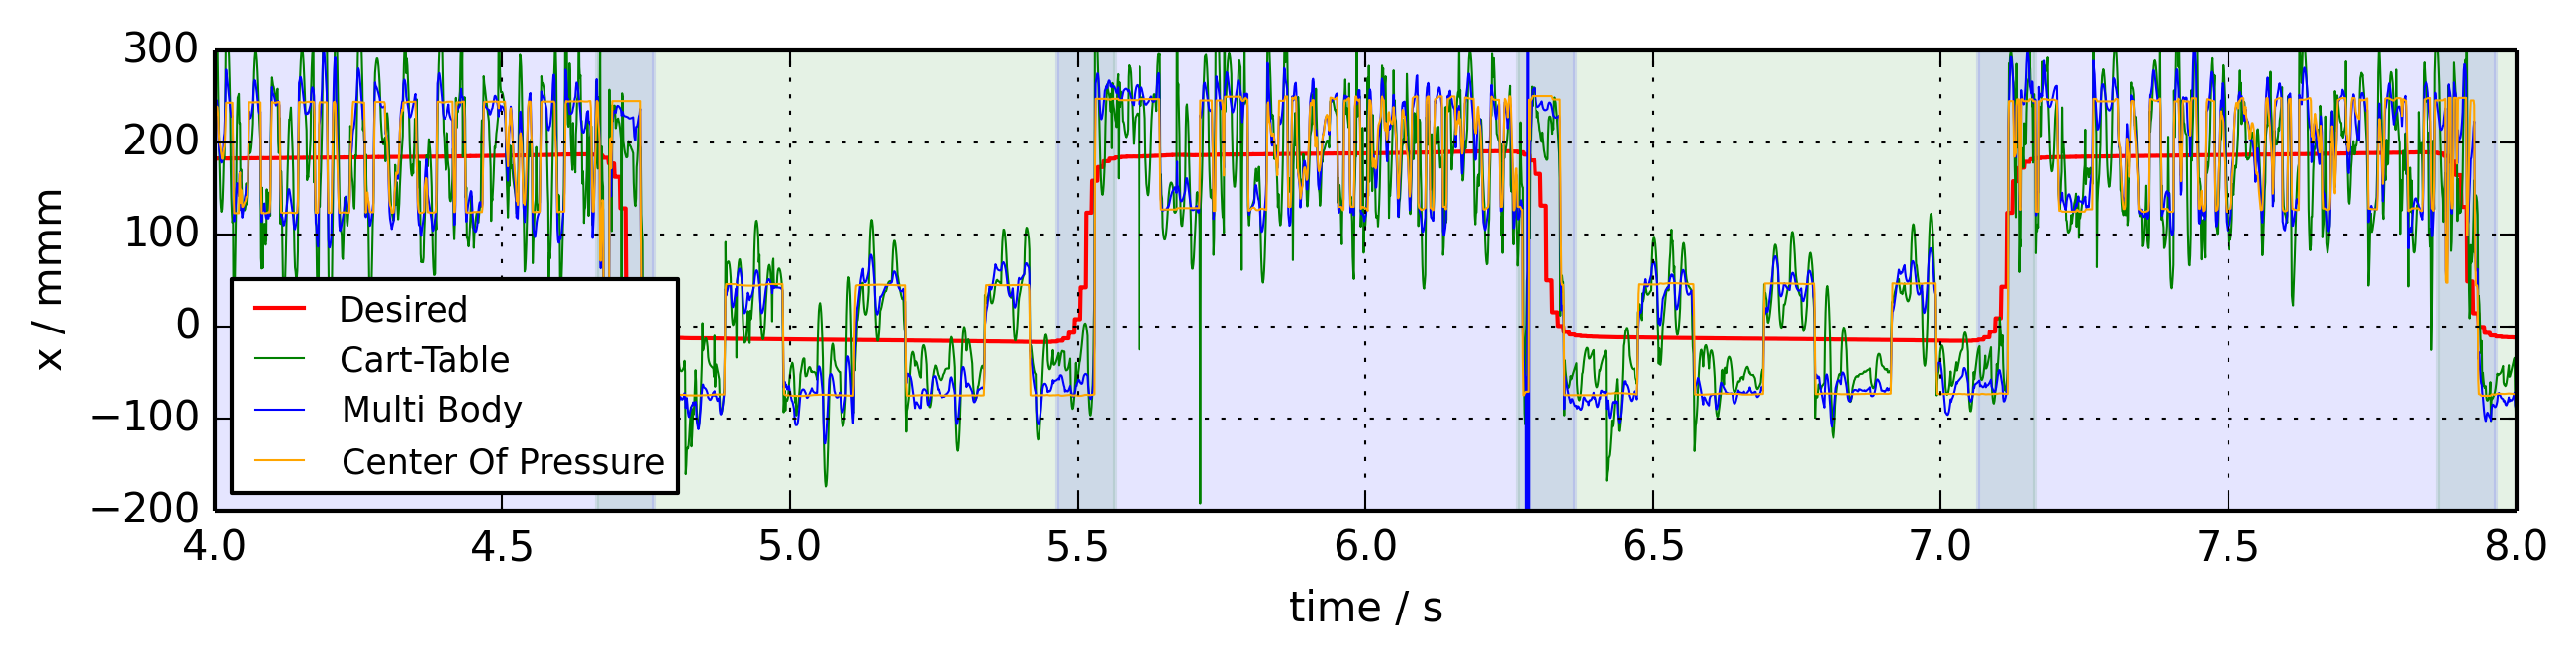
\includegraphics[width=\textwidth,resolution=300]{images/zmp_comparison.png}
\caption{Comparision of the Cart-Table and Multi-Body to estimate the realized ZMP during walking.}
\label{img:zmp-comparison}
\end{figure*}

\section{Simulating rigid body
dynamics}\label{section:rigid-body-simulation}

For physical simulation in general can be devided into discrete methodes
and continous methodes. Discrete simulators only compute the state of
the system at specific points in time, while continous simulators are
able to compute the state of the system at any point in time. While
contious simulation is the more flexible approach, it quickly becomes
impractical with the number of constrains involved. Typically a large
amount of differential equations need to be solved. Since it is hard to
obtain analytical solutions for most differential equations, numerical
methodes need to be used, which often have a large runtime. On contrast
discrete simulation methodes only compute simulation values for specific
time steps. This exploits the observation that we will typically query
the state of the physics engine only at a fixed rate anyway, e.g.~at
each iteration of our control loop). Rather than solving the differntial
equations that describe the physical system in each step, a solution is
derived from the previous simulation state.

A physical system we can typically find two kind of forces: Applied
forces and constraint forces. Applied forces are the input forces of the
system. Source of applied forces are for example objects like springs or
gravity. Constraint forces are fictious forces that arrise from
contrains we impose on the system: Non-penetration constraints, friction
constraints, position constrains of joints or velocity constrains for
motors. Mathematically we can express such constrains in the form:
$C(x) = 0$ or $\dot{C}(x) = 0$ in the case of equality constrains, or as
$C(x) \geq 0$ or $\dot{C(x)} \geq 0$ in the case of inequality
constrains. For example the position constraint of a joint $p$ connected
to a base $p_0$ with distance $r_0 = ||p-p_0||$ would be:
$C(p) = || p - p_0 ||^2 - r_0^2$ If $p$ is moving with a linear velocity
$v$ a constraint force $F_c$ is applied to $p$ to maintain this
constraint. We can view $C$ as a transformation from our cartesian space
to the constraint space. Thus by computing the jacobian $J$ of $C$ we
can relate velocities in both spaces. Furthermore we can realte
constraint space forces $\lambda$ with cartesian space forces using the
transpose of the Jacobian. Thus if we can find the constraint space
force $\lambda$ that is needed to maintain this constraint we can
compute $F_c$ using $F_c = J^T \lambda$. Computing this constraint space
forces is the task of the constraint solver.

The constrained solver used by \name{Bullet} and thus the constraint
solver used for simulating the patterns here is a sequential impulse
solver. To make some calculations easier, a SI solver works with
impulses and velocities rather than forces and accelerations. Impulses
and forces can be easily transformed in eachother as $P = F \cdot T$
where $P$ is the impulse and $T$ the timestep size. A sequential impulse
solver tries to compute the constraint force (in this case rather
impulse) $\lambda$ for each costraint \emph{seperately}. For each
constraint the following steps are executed:

\begin{enumerate}
\def\labelenumi{\arabic{enumi}.}
\itemsep1pt\parskip0pt\parsep0pt
\item
  Compute the velocity that results from \emph{applied forces} on the
  body
\item
  Calculate constraint force to satisfy the velocity constraint
\item
  Compute new velocity resulting from constraint force \emph{and}
  applied force on the body
\item
  Update position of the body by integrating velocity:
  $p[n+1] = p[n] + v \cdot T$
\end{enumerate}

Of course this might not lead to a global solution, as satisfying a
constraint might violate a previously solved one. The idea is to
repeadidetly loop over all constraints, so that a global solution will
be reached. Obviously the quality of this methode relies on how often
this loop is executed. Consider the case of a kinematic chain where a
movement of a link always violates at least one constraint. It is clear
that this methode needs a lot of iterations to yield good results in
this case. It becomes even worse in the case of a parallel kinematic
that is in contact with the ground, as is the case for a bipedal robot
in dual support stance. Solving a non-penetration constrain on either
end, will invalidate the position constraint of the next link. In turn,
the position constraint of each link needs to be updated until the other
end of the kinematic chain is reached. If the non-penetration constraint
is violated again for this end, the whole process starts again in
reverse direction. This leads to oscillations that need a lot more
iterations to level off to an acceptable level. Dispite these
inaccuracies using enought solver iteration this still yields an overall
usable systems. However the velocities still will have a small random
error in each simulation step. This poses a major problem when trying to
measure accelerations, as the random error acauses them to accelerate
wildly. This circumstance needs to be taken into account when dealing
with values derived from the acceleration (e.g.~the ZMP), as
mean-filters might be neccessary.

\chapter{Pattern generator}\label{pattern-generator}

To generate a walking pattern for a bipedal robot two basic approaches
are common:

\begin{enumerate}
\def\labelenumi{\arabic{enumi}.}
\item
  Generate (or modify) foot trajectories that realize a prescribed
  trajectory of the CoM
\item
  Generate a CoM trajectory for prescribed foot trajectories
\end{enumerate}

The first approach is generally used for implementing pattern generators
soley based on the 3D-LIPM model. \todo{citation needed}

The second approach is the more versatile one, since it is easy to
incorporate constrains of our environment (e.g.~only limited foot holds)
in the input of the pattern generator. However care must be taken while
chosing adequate step width and step length parameters for the foot
trajectory, so that they can actually be realized by the robot.

The pattern generator proposed by Kajita et al. \todo{add citation}
based on Preview Control realizes the second approach. We will discuss
the theoretical background of this pattern generator here in more
detail, since all pattern that we used where generated that way.

\section{Computing the CoM from a reference
ZMP}\label{computing-the-com-from-a-reference-zmp}

As we saw in the section \ref{section:table-cart} it is easy to compute
the resulting ZMP given the CoM and its acceleration. However for
generating the walking pattern, we want to compute the CoM trajectory
from a given ZMP. If you rearange the equations \ref{eq:zmp-x} and
\ref{eq:zmp-y} you see that we have to solve a second order differential
equations:

\begin{equation} \label{eq:com-x}
c_x = \frac{z_c}{g} \cdot \ddot{c_x} + p_x
\end{equation}

\begin{equation} \label{eq:com-y}
c_y = \frac{z_c}{g} \cdot \ddot{c_y} + p_y
\end{equation}

There are several ways to solve this differential equations, for example
by transforming them to the frequency-domain. This however would mean,
the ZMP trajectory needs to be transformed to the frequency domain as
well, e.g.~using Fast Fourier Transformation. This has two main
problems:

\begin{enumerate}
\def\labelenumi{\arabic{enumi}.}
\item
  It has a significant computational overhead. (For FFT the additional
  runtime would be in $O(n \log n)$)
\item
  We need to know the whole ZMP trajectory in advance.
\end{enumerate}

Instead Kajita et. al. chose to define a dynamic system in the time
domain that describes the CoM movement.

\subsection{Pattern generation as dynamic
system}\label{pattern-generation-as-dynamic-system}

\todo{maybe do a formal introduction into dynamic system and the state space approach}

For simplicity we will only focus on the dynamic description of one
dimension, as the other one is analogous. To transform the equations to
a strictly proper dynamical system, we need to determine the state
vector of our system. For the table-cart model it suffices to know the
position, velocity and acceleration of the cart. Thus the state-vector
is defined as $x = (c_x, \dot{c_x}, \ddot{c_x})$. We can define the
evolution of the state vector as follows:

\begin{equation} \label{eq:dyn-system}
\frac{d}{dt} \left(\begin{array}{c}
c_x \\
\dot{c_x} \\
\ddot{c_x} \\
\end{array} \right)
=
\overbrace{
\left(\begin{array}{ccc}
0 & 1 & 0\\
0 & 0 & 1 \\
0 & 0 & 0 \\
\end{array}\right)
}^{ =: A_0}
\cdot
\left(\begin{array}{c}
c_x \\
\dot{c_x} \\
\ddot{c_x} \\
\end{array}\right)
+
\overbrace{
\left(\begin{array}{ccc}
0 & 0 & 0\\
0 & 0 & 0\\
1 & 0 & 0\\
\end{array}\right)
}^{ =: B_0}
u
\end{equation}

As you can see the jerk of the CoM was introduced as an input
$u_x = \frac{d}{dt} \ddot{c_x}$ into the dynamic system.

We use equation \ref{eq:zmp-x} to calculate the actual output of the
dynamic system the resulting zmp, that will be controlled:

\begin{equation} \label{eq:zmp-x-output}
p_x =
\left(\begin{array}{ccc}
1 & 0 & \frac{-z_c}{g} \\
\end{array}\right)
\cdot
\left(\begin{array}{c}
c_x \\
\dot{c_x} \\
\ddot{c_x} \\
\end{array}\right)
\end{equation}

Using this formulation of the dynamic system we need to derive the
evolution of our state vector using the state-transition matrix. Since
our input ZMP trajectory will consist of discrete samples at equal time
intervals $T$ we define the discrete state as $x[k] := x(k \cdot T)$.
Please note that this system is a linear time-invariant system (LTI),
and both matrices $A_0$ and $B_0$ are constant. We can therefore use the
standart approach to solve this system using the equation:

\begin{equation}
x(t) = e^{A_0 \cdot (t - \tau)} x(\tau) + \int^t_\tau e^{A_0 \cdot (t - \lambda)} B_0 u(\lambda) d\lambda
\end{equation}

In our discrete case that becomes:

\begin{eqnarray} \label{eq:state-transition-discrete}
x[k+1] & = & e^{A_0 \cdot ((k+1)T - kT)} x[k] + \int^{(k+1)T}_{kT} e^{A_0 \cdot ((k+1)T - \lambda)} B_0 u(\lambda) d\lambda \\
       & = & e^{A_0 \cdot T} x[k] + \left(\int^{(k+1)T}_{kT} e^{A_0 \cdot ((k+1)T - \lambda)} d\lambda \right) \cdot B_0 u[k]\\
       & = & e^{A_0 \cdot T} x[k] + \left(\int^{0}_{T} e^{A_0 \cdot \lambda} d\lambda\right) \cdot B_0 u[k]
\end{eqnarray}

Keep in mind that $u(\lambda) = u[k], \lambda \in (kT, (k+1)T)$ so we
can move it outside of the integral. Let us first compute a general
solution for the matrix exponential $e^{A_0 \cdot t}$. It is easy to see
that $A_0$ is nilpotent and $A_0^3 = 0$, thus the computation simpilfies
to the following:

\begin{equation}
e^{A_0 t} := \sum^{\infty}_{i=0} \frac{(A_0 \cdot t)^i}{i!} = I + A_0 \cdot t + A_0^2 \cdot \frac{t^2}{2} + 0
=
\left(\begin{array}{ccc}
1 & t & \frac{t^2}{2}\\
0 & 1 & t \\
0 & 0 & 1 \\
\end{array}\right)
\end{equation}

Using this solution computing the integral in
\ref{eq:state-transition-discrete} is quite easy:

\begin{equation}
\int^{0}_{T} e^{A_0 \cdot \lambda} d\lambda =  -\int^{T}_{0} \left(\begin{array}{ccc}1 & t & \frac{t^2}{2}\\0 & 1 & t\\ 0 & 0 & 1\end{array}\right) dt
                                            =  -\left.\left(\begin{array}{ccc} %
                                                          t & \frac{t^2}{2} & \frac{t^3}{6} \\ %
                                                          0 & t             & \frac{t^2}{2} \\ %
                                                          0 & 0             & t %
                                                 \end{array}\right)\right|_{0}^{T}\\
                                            =   \left(\begin{array}{ccc} %
                                                          T & \frac{t^2}{2} & \frac{T^3}{6} \\ %
                                                          0 & T             & \frac{T^2}{2} \\ %
                                                          0 & 0             & T %
                                                \end{array}\right)
\end{equation}

Substituting the results in \ref{eq:state-transition-discrete} yields:

\begin{eqnarray} \label{eq:state-transition-result}
x[k+1] & = &  \overbrace{\left(\begin{array}{ccc} %
                     T & \frac{t^2}{2} & \frac{T^3}{6} \\ %
                     0 & T             & \frac{T^2}{2} \\ %
                     0 & 0             & T %
               \end{array}\right)}^{=: A} x[k]
             + \overbrace{\left(\begin{array}{ccc} %
                      \frac{T^3}{6} \\ %
                      \frac{T^2}{2} \\ %
                      T %
               \end{array}\right)}^{=: B} \cdot u_x[k]
\end{eqnarray}

\subsection{Controlling the dynamic
system}\label{controlling-the-dynamic-system}

To control this dynamic system we need to determine an adequate control
input $u_x$ to realize the reference ZMP trajectory. A performence index
$J_x$ for a given control input $u_x$ is needed to formalize what a
``good'' control input would be. A naive performence index could be:

\begin{equation}
J_x[k+1] := (p^{ref}_x[k+1] - p_x[k+1])^2
\end{equation}

To minimize it, we need to find $u_x$ for which $p_x = p^{ref}_x$. By
substituting $p_x[k+1]$ with \ref{eq:zmp-x-output} and $x[k+1]$ with
\ref{eq:state-transition-result} this yields:

\begin{equation}
u_x[k] = \frac{p^{ref}_x[k+1] - C \cdot A \cdot x[k]}{C \cdot B} = \frac{p^{ref}_x[k+1] - (1, T, \frac{1}{2} T^2 -\frac{z_c}{g}) \cdot x[k]}{\frac{1}{6}T^3 - \frac{z_c}{g} T}
= \frac{p^{ref}_x[k+1] - p_x[k] - T \dot{c_x}[k] - \frac{1}{2} T^2 \ddot{c_x}[k]}{\frac{1}{6}T^3 - \frac{z_c}{g} T}
\end{equation}

To analyse the behaviour of this control law for $u_x$ we simulate the
rapid change of reference ZMP when changing the support foot.
\todo{insert plot}

As you can see the reference ZMP is perfectly tracked. However, the CoM
does not behave as expected. To achive the required ZMP position the CoM
will be \emph{accelerated indefinietly} in the opposite direction.
Clearly this is not desired and will lead to falling on a real robot. A
more sophisticated performence index is needed. To eventually reach a
stable state at which the CoM comes to rest, the performence index
should include a state feedback. Also note the large jerk that is
applied to the system when the reference ZMP position changes rappidly.
In a real mechanical system large jerks will lead to oszillations, which
will disturbe the system. Thus the performence index should also try to
limit the applied jerk.

Another problem is caused by the very nature of a controller: The
controller starts to act \emph{after} we have a deviation from our
reference ZMP trajectory. Trying make this lag as small as possible can
lead to very high velocities, which might not be realizable by motors of
a robot. However we have at least limited knowledge of the future
reference trajectory. This knowledge can be leveraged by using Preview
Control, which considers the next $N$ timesteps for computing the
performence index.

\todo{add citation katayama} Kajita et. al. use a performence index
proposed by Katayama et. al. to solve all of the problems above:

\begin{equation}
J_x[k] = \sum^{\infty}_{i=k} Q_e e[i]^2 + \Delta x[i]^T Q_x \Delta x[i] + R \Delta u_x[i]^2
\end{equation}

$Q_e$ is the error gain, $Q_x$ a symmetric non-negative definite matrix
(typically just a diagonal matrix) to weight the components of
$\Delta x[i]$ differently and $R > 0$. Conveniently Katayama also
derived an optimal controller for this performence index, which is given
by:

\begin{equation}
u[k] = -G_i \sum^k_{i=0} e[k] - G_x x[k] - \sum^N_{j=1} G_p p^{ref}_x[k + j]
\end{equation}

The gains $G_i, G_x, G_p$, can be derived from the parameters of the
performence index. Since the calculation is quite elaborate we refer to
the cited article by Katayama p.~680 for more details.

\section{Implementation}\label{implementation}

\todo{block diagramm of architechture} To generate walking patterns
based on the ZMP preview control methode, the approach from Kajita was
implemented in \name{libBipedal} a shared library. A front-end was
developed to easily change parameters, visualize and subsequently export
the trajectory to the \name{MMM} format. The implementation was build on
a previous implementation, which was refactored, extended and tuned with
respect to results from the dynamics simulation.

The pattern generator makes extensive usage of
\name{Simox VirtualRobot}, for providing a model of the robot and the
associated task of computing the forward- and inverse kinematics.

Generating a walking pattern consists of multiple steps. First the foot
positions are calculated. These are used to derive the reference ZMP
trajectory which is feed into the zmp preview controller. From that the
CoM trajectory is computed. The CoM trajectory and feet trajectories are
then used to compute the inverse kinematics. The resulting joint
trajectory is displayed in the visual front-end and can be exported.
Each step is contained in dedicated modules that can be easily replaced,
if needed. We will outline the implementation of each module seperately.

\subsection{Generating foot
trajectories}\label{generating-foot-trajectories}

To generate the foot trajectories several parameters are needed:

\todo{table with used parameters}

\begin{description}
\item[Step height $h$]
Maximum distance between the foot sole and the floor
\item[Step length $l$]
Distance in anterior direction ($y$-Axis) between the lift-off point and
the touch-down point
\item[Step width $w$]
Distance in lateral directoin ($x$-Axis) between both TCP on the feet
\item[Single support duration $t_{ss}$]
Time the weight of the robot is only support by exactly one foot
\item[Dual support duratoin $t_{ds}$]
Time the weight of the robot is supported by both feet
\end{description}

\subsubsection{Walking straight}\label{walking-straight}

Since the foot trajectories of a humanoid walking have a cyclic nature,
we only need three different foot trajectories that can be composed to
arbitrarily long trajectories: Two transient trajectories for the first
and last step respectively and a cyclic motion that can be repeated
indefinetly. We can use the same trajectories for both feet, as they are
geometrically identical. Each foot trajectory starts with swing phase
and a resting phase. The trajectory in $y$ and $z$ direction is computed
by a 5th order polynomial that assures the velocities and accelerations
are approaching zero at the lift-off and touch-down point. The first and
last step only have half of the normal step length, since the trajectory
is starting and ending from a dual support stance, where both feet are
placed parallel to eachother. Each trajectory is encoded as a
$6 \times N$ matrix, each column containing cartesian coordinates and
roll, pitch and yaw angles.

\subsubsection{Walking on a circle}\label{walking-on-a-circle}

Much of the general structure of the foot trajectory remains the same as
for walking straight. However instead of specifing the step length, it
is implicitly given by the segment of the cricle that should be
traversed and the number of steps. So extra care needs to be taken to
specify enough steps so that the generated foot positions are still.
Each foot needs to move on a circle with radius
$r_{inner} = r - \frac{w}{2}$ or $r_{outer} = r + \frac{w}{2}$ depending
which foot lies in the direction of the turn. The movement in
$z$-direction remains unaffected. However the movement in the $xy$-plane
is transformed to follow the circle for the specific foot.
\todo{Current implementation does effectively that, but is actually a hack. Needs seperate trajectories for left/right}
The same polynomial that was previously used for the $y$-direction is
now used to compute the angle on the corresponding circle and the $x$
and $y$ coordinates are calculated acordingly. The foot orientation is
computed from the tangential (y-Axis) and normal (x-Axis) of circle the
foot follows.

\subsubsection{Balancing on one foot}\label{balancing-on-one-foot}

To test push recovery from single support stance a special pattern was
needed. To generate this another footstep planer was implemented that
generates a trajectory for standing on one foot. Starting from dual
support stance, the swing leg is moved in vertical direction until the
usual step height is achieved. Additionally the foot is moved in lateral
direction to half the step width. This reduces the necessary upper body
tilt to compensate the inbalance. For the last step the inverse movement
is performed to get back into dual support stance. This methode could be
extended to walk by setting the next support foot in a straight line
before the current support foot. The swing foot would need to be moved
in an arc in lateral direction to avoid self-collisions.
\todo{It is easy to extent this: DO IT.}

\subsection{ZMP reference generation}\label{zmp-reference-generation}

As an input for the ZMP preview control, we need a reference ZMP
movement that corresponds with the foot trajectory. The reference
generator receives a list of intervals associated with the desired
support stance and foot positions as input. In single support phase, the
reference generator places the ZMP in the center of the support polygone
of the corresponding foot. Since the support polygone is convex, the
center is the point furthest away from the border of the polygone. Thus
it should guarantee a maxium of stability with regard to possible ZMP
errors. In dual support phase, the reference generator shifts the ZMP
from the previous support foot to the next support foot. Kajita et. al.
suggest using a poylnomial to interpolate the ZMP positions between the
feet. However a simple step function
$\sigma(t) = \left\{\begin{array}{lr}p_1 & t \leq t_0 \\ p_2 & t > t_0 \end{array}\right.$
seems to suffice as well. Since the the touch-down of the swing foot
might have a small lag, it is important that $t_0$ is the middle of the
dual support phase. This assures we do not start to move the ZMP too
early.

\subsection{ZMP Preview Control}\label{zmp-preview-control}

This module implements the methode described by Kajita et. al. and uses
the methode outlined by Katayama et. al. to compute the optimal control
input $u[k]$. Since it is computational feasable, the preview periode
consists of the full reference trajectory. For an online usage of this
methode, this could be reduced to a much smaller sample size.
\todo{Add timings, implement configurable preview periode} Using the
system dynamics described by \ref{eq:state-transition-result} the CoM
trajectory, velocity and acceleration can be computed. The
implementation makes heavy use of Eigen, a high performence linear
algebra framework that uses SIMD instructions to speed up calculations.
Thus thus a calculation time of \fixme{calculation time} could be
achieved.

\subsection{Inverse Kinematics}\label{inverse-kinematics}

Using the foot trajectories and CoM trajectory the actual resulting
joint angles need to be calculated. Since the kinematic model that is
used has a total of \fixme{DOF} degrees of freedom, we need to reduce
the number of joints that are used to a sensible value. For walking only
the joints of the legs and both the torso roll and pitch joints are
used. All other joints are constrained to static values that will not
cause self-collisions (e.g.~the arms are slightly extended and do not
touch the body). For comptuing the IK additional constraints where
added, to make sure the robot has a sensible pose: The chest should
always have an upright position and the pelvis should always be parallel
to the floor. To support non-straight walking, the pelvis and chest
orientation should also follow the walking direction. Thus the following
methode to compute the desired chest and pelvis orientation is used:

\begin{enumerate}
\def\labelenumi{\arabic{enumi}.}
\item
  Compute walking direction $y'$ as normed mean of y-Axis of both feet:
  $y' := \frac{y_{left} + y_{right}}{|y_{left} + y_{right}|}$
\item
  Both should have an upright position $z' := (0, 0, 1)^T$
\item
  Compute $x'$ as the normal to both vectors: $x' := y' \times z'$
\item
  Pose $R'$ is given by $R' = (x', y', z')$
\end{enumerate}

A special property of the model that was used for computing the inverse
kinematics, is that TCP of the left leg was chosen as root node. Since
we can specify the root position freely, that removes the need of
solving for the left foot pose. Thus the following goals need to be
satisfied by the inverse kinematics:

\begin{enumerate}
\def\labelenumi{\arabic{enumi}.}
\item
  Chest orientation
\item
  Pelvis orientation
\item
  CoM position
\item
  Right foot pose
\end{enumerate}

To solve the inverse kinematics a hiearchical solver was used to solve
for that goals in the given order. It was observed that specifing a good
target height for the CoM is of utmost importance for the quality of the
IK. Specifing the CoM height too height or too low can lead to the
effective loss of degrees of freedom.

\todo{Maybe a more theoretical explaination?}

\subsection{Trajectory Export}\label{trajectory-export}

The trajectory was exported in open \name{MMM} trajectory format. The
format was extended to export additional information useful for
debugging and controlling the generated trajectory. That means besides
the joint values and velocites the trajectory also includes the CoM and
ZMP trajectory that was used to derive them. Also information about the
current support phase is saved. For convinience the pose of chest,
pelvis, left and right foot are exported as homogenous matrices as well.
This was done to save the additional step of computing them again from
the exported joint trajectory for the stabilizer and also reduce an
additional error source.

\todo{Maybe doing the FK now would be better and more versatile, since we could feed normal \name{MMM} trajectories in the stabilizer}

\section{Dynamic simulation}\label{dynamic-simulation}

To evaluate the generated trajectories a simulator for the dynamics was
developed. The simulator was build on the \name{SimDynamics} framework
that is part of \name{Simox}. \name{SimDynamics} uses Bullet Physics as
underlying physics framework. A big part of the work on the simulator
was spend on configuring the parameters and finding flaws in the physics
simulation. Thus the simulator includes a extensive logging framework
that measures all important parameters of the simulation. For visulizing
and analysing the measurement the Open Source tools \name{IPython},
numpy and \name{pandas} where used.

\subsection{Practical challenges of physics
simulation}\label{practical-challenges-of-physics-simulation}

While walking only the feet of the robot are in contact with the ground.
Thus the stability of the whole robots depends on the contact of the
feet with the floor. Especially in single support phase that area is
very small with regard to the size of the robot. For that reason the
accuracy of ground contatc forces and friction is of utmost importance
for the quality of the simulation. In general three classes of errors
need to be elimnated to get a good simulation:

\begin{enumerate}
\def\labelenumi{\arabic{enumi}.}
\item
  Incorrectly configured parameters, such as fictions coefficent and
  contact thresholds
\item
  Numerical errors
\item
  Inherent errors of the methode
\end{enumerate}

As outline in the section about discrete time dynamic simulation, the
physics of the system are formulated as input forces and constrains that
need to be solved for the constraint forces. Since bullet uses an
iterative approach that solves each constraint independently, it is of
utmost importance to use a sufficient amount of iterations for each
simulation step. Another important parameter is the timestep of each
simulation step. Through experimental evaluation a simulation with 2000
solver iterations and a timestep size of 1ms was sufficiently stable.
However since the number of iterations is very high and a lot of
timesteps are calculated during the simulation, numeric errors become
significant. That made is neccessary to enable using double precision
floating point numbers for the values used during simulation.

To decide which contact constrains are active for which points, Bullet
must solve for object collisions. Depending on the objects involved
different algorithms are used to calculate the contact points. Major
gains in accuracy could be observed by replacing the feet and the floor
with simple box shapes, instead using mesh based models.

\subsection{Simulating walking
patterns}\label{simulating-walking-patterns}

The simulator was designed to load arbitrary motions in the \name{MMM}
format and replay them. Additional stabilization algorithms can be
applied depending on additional information provided in the \name{MMM}
motions.
\todo{Make sure you can really load vanilla \name{MMM} trajectories without crashing}

Even during simple playback of a trajectory, a number of conisderations
due to the dynamics need to be taken into account. We will outline some
of the problems and how they where resolved.

Simply applying the joint values at the given point in time, will lead
to large jumps in velocity, acceleration and jerk. This will cause large
oscillations, which in turn result in destabilizing disturbances.
Interpolation between the joint angles of two frames can mitigate this.
To implement this cubic splines where used instead of linear
interpolation, as they also ensure that the velocity is continous.

Disturbances due to the simulation will cause position errors in the
joints. To fix that PID based motor controllers were added to
\name{SimDynamics}. They control the motor velocites to compensate
position errors.

Since the motors used by the simulation framework are velocity
controlled, their acceleration is not limited. This is not consistent
with real motors, thus limits for velocites and acceleration where
introduced to \name{SimDynamics}, that can be configured on a per-joint
basis.

An important part of the simulation is the generation of measurements
that can saved to be carefully evaluted offline or displayed in the
visualization. For this purpose a modular measuremt component was added
to the simulator. An important design goal was to keep the measurement
component as simple to extend and maintain as possible. Each module
meassures a specific set of values and writes them, indexed by the
corresponding timestamp, to its log file. As output format the well know
plaintext format CSV was used. The visualization can query the
measurement components directly to get the newest values to be
displayed. For example the ZMP module measures the actual ZMP and also
provides an interface to query the trajectory ZMP and the reference ZMP
that was provided as input for the pattern generator. Thus all three
values can be displayed in the visualization and easily compared later
by analysing the log file. Since the goal was to keep the component as
simple as possible, we use exsistening well known tools for analysing
the generated log files. Some small helper scripts are provied to make
it easier to load the data into the time series analysis framework
\name{pandas}. \name{Pandas} interfaces with the popular plotting
framework \name{matplotlib} to diplay plots of the data. \name{IPython}
is used to easily run the analysis and display the results in a browser
window. All plots of simulated patterns found in this thesis can be
generated automatically for every simulation.

\todo{Screenshot of analysis software}

\chapter{Stabilizing a trajectory}\label{stabilizing-a-trajectory}

\todo{More introduction: Most stabilizers are propritary and very robot specific.}

While executing a trajectory there are several sources of errors that
will make it neccessary to correct the trajectory. We can devide them in
about three main classes:

\begin{description}
\item[Disturbances of the environment:]
Pattern generator make some assumptions about the environment they
operate in. Most prominently the 3D-LIMP assumes the floor is completely
flat and has no slope. Also we assume we can navigate without colliding
with other object. Any environment that deviates from this assumption
can be seen as a disturbance.
\item[Disturbances due to simulation errors:]
Physical simulations often make a tradeoff between speed and simulation
accuracy. Thus the simulation might not always behave as it was modeled
during calculating the pattern, or as it would behave in reality.
\item[Disturbances due to errors of the methode:]
Often pattern generators use simplified models of the dynamics involved
to derive generation scheme. For example the pattern generator that was
used here assumes the ZMP behaves as the cart-table-model predicts.
However the real ZMP calculated from the multi-body dynamics can
substantially deviate.
\end{description}

\section{Controlling a deviation}\label{controlling-a-deviation}

When using a ZMP based control scheme to derive a walking pattern it
seems natural to check for deviations of the actual ZMP from the goal
ZMP. However a deviation from the reference ZMP does not neccessarily
mean we will see any disturbance. As long a the ZMP remains inside the
support polygone the trajectory can be executed as planed. Also we saw
before, it is entirely possible to realize the reference ZMP while being
in an overall state that deviates significantly from the state we
assumed while generating the pattern. Thus we also need to check for a
diviation in the trajectory of our CoM. A common approach to correct for
CoM position is to control the pose of the chest frame of the robot.
This only works if the majority of the mass of a robot is located in the
upper body and arms. Luckily for most humanoid robots this is the case.

\section{Stabilizer}\label{section:stabilizer}

We chose a stabilizer proposed by Kajita et. al. in their 2010 paper.
\todo{add reference}. The stabilizer only needs a joint trajectory of
the walking pattern augmented with a desired ZMP trajectory. This allows
the stabilizer to use patterns that where generated synthetically,
e.g.~by a pattern generator, or patterns that are the results of
(adapted) motion capturing. The methode proposed by Kajita does not need
a torque controlled robot, but works with position control. This was
very important for the selection of this stabilizer as, the motors in
\name{Bullet} are velocity controlled, thus we can not controll the
torque directly.

The controller works by attaching control frames to specific points on
the robot. The reference position of this frames can be calculated from
the input trajectory using forwards kinematics. To compensate a
disturbance the orientation of a reference frame is modified. The
modified reference frames are then converted to the modified joint
angles by the inverse kinematics.

\todo{include block digramm of controller}

In the remainder of this chapter we will use the superscript $d$ to
denote reference values and the subscript $*$ to denote modified values.

For this approach four control frames where selected. The chest to
modify the body posture, the feet to modify the ankle torque, and the
pelvis to modify the difference between contact forces of the two feet.

\subsection{Controlling the body
posture}\label{controlling-the-body-posture}

The control strategy of the chest pose is straight forward: Given the
reference roll angle $\phi^d$ and reference pitch angle $\theta^d$
compute the differences to the actual angles $\phi$ and $\theta$. The
main problem in a real robot is to obtain the actual global pose of this
frame. The proposed methode is to use a Kalman filter to estimate the
pose from the joint position and accelerometers. We did not implement
this methode in simulation, as it is easy to obtain the exact pose from
the simulator. To prevent rapid movements of the chest that cause large
accelerations, a dampening controller is used. The angles $\Delta \phi$
and $\Delta \theta$ can be calculated by the following equations:

\begin{equation}
\Delta \dot{\phi} = \frac{1}{D_c} (\phi^d - \phi) - \frac{1}{T_c} \cdot \Delta \phi
\end{equation}

\begin{equation}
\Delta \dot{\theta} = \frac{1}{D_c} (\theta^d - \theta) - \frac{1}{T_c} \cdot \Delta \theta
\end{equation}

$D_c$ describes the dampening gain. $T_c$ is constant that describes how
long it will take to reach the normal positions $\Delta \phi = 0$ and
$\Delta \theta = 0$ respectively if there is no error.

The modified reference frame $R^{d*}_c$ can the be calculated by
rotating the reference frame by the additional angles:

\begin{equation}
R^{d*}_c = R^d \cdot R_{RPY}(\Delta \phi, \Delta \theta, 0)
\end{equation}

To get an idea how this controller compensates CoM inaccuracies consider
the case where the upper body is bent forward. Since our reference
trajectory specifies an upright upper body pose we can assume that
$\phi^d = 0$. Since the upper body is bent forward the roll angle $\phi$
will be below zero. Depending on $D_c$ we will eventually reach
$\Delta \phi \approx |\phi|$, thus the reference frame will be modified
to bent backwards to compensate the wrong pose.

\subsection{Controlling the ankle
torques}\label{controlling-the-ankle-torques}

Since the stabilizer only has the joint trajectory and desired ZMP
trajectory as input, we need a way to compute the desired actuation
torques on the ankles. The canonical way to do this, would be to solve
the inverse dynamics of the robot. However for this we need an acurate
model of the robot, including correct masses and moments of intertia for
each link. This model is not always easy to obtain and calculating the
inverse dynamics of a robot with many degrees of freedom is rather slow.
For this reason a simple heuristic is proposed to yield approximate
torques given a reference ZMP position. However in the single support
phase it is easy to calculate the \emph{exact} actuation torque on the
ankle, that is required to realize the given reference ZMP.

First we need to calculate the force in $z$-direction applied on the
foot at the ankle $p_{ankle}$ which we name $f_g$ by:

\begin{equation}
f_g = M \cdot g
\end{equation}

Where $g$ is the gravity vector and $M$ the mass of the robot. Given
$f_g$ acting on the ankle position $p_{ankle}$ we can obtain the ankle
torque in single support phase easily using the fact, that the torque
around the ZMP is zero:

\begin{equation}
\begin{array}{lcccr}
\tau_{zmp} & = & (p_{ankle} - p^d_{zmp}) \times f_g & + & \tau^d_{ankle} \\
0 & = & (p_{ankle} - p^d_{zmp}) \times f_g & + & \tau^d_{ankle} \\
\tau^d_{ankle} & = & -(p_{ankle} - p^d_{zmp}) \times f_g & & \\
\end{array}
\end{equation}

In dual support phase however that matter is more complicated. Since
both feet are in contact with the ground, the weight of the robot is
distributed between them. If we take the forces $f_R$ and $f_L$ which
act on the right ankle $p_R$ and left ankle $p_L$ respectively we know
that $f_R + f_L = f_g$. Thus there exists $\alpha \in [0, 1]$ for which:
$f_R = \alpha \cdot f_g$ and $f_L = (1-\alpha) \cdot f_g$. A heuristic
for computing this alpha is the \emph{ZMP distributor}.

\todo{For some reason I named the class ForceDistributor, I should fix that}

The idea is to calculate the nearest points $p_{L\#}$ and $p_{R\#}$ from
the ZMP to the support polygones of the feet. If the ZMP falls inside
one of the support polygones set $\alpha = 1$ or $\alpha = 0$
respectively. If it is outside of bothe support polygones the ZMP is
projected onto line from $p_{L\#}$ to $p_{R\#}$ yielding the point
$p_{\alpha}$.

We can then set $\alpha$ to:

\begin{equation}
\alpha = \frac{|p_{\alpha} - p_{L\#}|}{|p_{R\#} - p_{L\#}|}
\end{equation}

If $\tau_L$ and $\tau_R$ are the torques in the left and right ankle
respectively, we can calculate the torque around the ZMP as:

\begin{equation} \label{eq:ds-torque}
\tau_{zmp} = (p_R - p^d_{zmp}) \times f_R + (p_L - p^d_{zmp}) \times f_L + \tau^d_L + \tau^d_R
\end{equation}

As before, we assume that $\tau_{zmp} = 0$ which lets us solve
\ref{eq:ds-torque} for $\tau_0 := \tau^d_L + \tau^d_R$:

\begin{equation} \label{eq:tau0-torque}
\tau_0 = (p_R - p^d_{zmp}) \times f_R + (p_L - p^d_{zmp}) \times f_L
\end{equation}

\todo{define ground frame} We now again apply a heurstic using the
$\alpha$ computed before to distribute $\tau_0$ to each ankle. First we
need to transform $\tau_0$ from the global coordinate system to a local
coordinate system described by the \emph{ground frame}. We mark all
vectors in the local coordinate system with $'$. The heuristic applied
is: The torque around the $x$-Axis in each ankle is approximately
proportional to the force applied at that ankle. Thus:

\begin{equation} \label{eq:torque-right-x}
\tau^{d'}_{Rx} = \alpha \tau_{0x}'
\end{equation}

\begin{equation} \label{eq:torque-left-x}
\tau^{d'}_{Lx} = (1-\alpha) \tau_{0x}'
\end{equation}

The torque around the $y$-Axis depends on the direction of the total
torque $\tau_{0y}'$. If the total torque acts in clockwise direction
(negative sign), we can assume it will only be applied to the left foot.
If the torque acts in anti-clockwise direction (positive sign), we
assumte it will only be applied to the right foot.

\begin{equation} \label{eq:torque-right-x}
\tau^{d'}_{Ry} = \left\{
\begin{array}{lr}
\tau_{0y}', & \tau_{0y'} > 0 \\
0, & else
\end{array}
\right.
\end{equation}

\begin{equation} \label{eq:torque-left-x}
\tau^{d'}_{Ly} = \left\{
\begin{array}{lr}
\tau_{0y}', & \tau_{0y'} < 0 \\
0, & else
\end{array}
\right.
\end{equation}

We can now transform the torques form our local coordinate system to the
coordinate system of the corresponding foot yielding $\tau^d_L$ and
$\tau^d_R$.

\todo{Cite kajita paper from 2005 that outlines the motivation for doing pose control}

Now that we have obtained the reference torques, we can try to control
the torque in each angle using the measured torques $\tau_R$ and
$\tau_L$. However since we assume a position controlled robot, the
torque differences need to be translated into pose changes. There are
three primary cases that need to be considered if we change the
reference pose of a foot:

\todo{image with springs}

\begin{description}
\item[The foot is not in contact with the ground:]
Changing the reference pose will just affect the foot
\item[The foot is in contact with the ground, but the contact is
non-solid:]
If the foot has a soft contact surface (e.g.~rubber) we can model the
contact with the ground as springs that connect the ground with the
contact points on the foot. Changing the pose of the foot will
relax/compress the springs and change the contact forces acoordingly.
\item[The foot is in solid contact with the ground:]
Changing the reference foot pose \emph{will not change the foot pose at
all}. Instead, the pose of the rest of the robot is changed. If the foot
pose is changed by the angles $\Delta \phi$ and $\Delta \theta$ all
other frames of the robot will be changed by $-\Delta \phi$ and
$-\Delta \theta$.
\end{description}

\todo{IK model <-> real robot}

For a foot with a rubber surface we will start with a non-solid contact
and transition to a solid contact, once the rubber is sufficiently
compressed.

To get an idea how changing the pose on such a foot with rubber surface
affects the torque, consider the case of rotating the foot around its
lateral axis (x-Axis) in anti-clockwise direction. Since the contact
with the ground is at first non-solid, we can employ the spring model.
The springs at the front of the foot are compressed thus the force
applied at the corresponding contact points increases. Accordingly the
springs at the back are compressed less, thus the force applied to the
corresponding contact points decreases. Resulting we see a increase in
torque around the $x$-Axsis.

If the springs are compressed sufficiently, we can assume the contact
with the floor is solid. Since the pose of the foot does not change, the
increase in the joint angle in the ankle will rotate the upper body
backwards. Recall the 3D-LIMP model for a moment, in that model this
means our pendulum swings backwards. This will lead to an increase of
the torque around the $x$-Axis in the base of the pendulum, the ankle
joint.

For rotating the foot around the $y$-axis the same ideas hold.

As a result we see that additional foot rotation long the $x$- and
$y$-Axis have a proportional relationship with the torque around that
axis. This motivates the definition of the controller proposed by Kajita
et. al. The additional rotation angles are can be calculated by the
following equations:

\todo{Maybe add a step response to the controller}

\begin{equation}
\Delta \dot{\phi_i} = \frac{1}{D_{ix}} (\tau^d_{ix} - \tau_{ix}) - \frac{1}{T_{ix}} \cdot \Delta \phi_i
\end{equation}

\begin{equation}
\Delta \dot{\theta_i} = \frac{1}{D_{ix}} (\tau^d_{iy} - \tau_{iy}) - \frac{1}{T_{ix}} \cdot \Delta \theta_i
\end{equation}

Where $i \in \{R, L\}$. This again utilizes the same concept of a
dampening controller that was used previously for controlling the chest
frame orientation. We can use the obtained angles $\Delta \phi_i$ and
$\Delta \theta_i$ to compute the modified reference frames for the feet:

\begin{equation}
R^{d*}_i = R^d_i \cdot R_{RPY}(\Delta \phi_i, \Delta \theta_i, 0)
\end{equation}

\subsection{Foot force difference
controller}\label{foot-force-difference-controller}

In the previous section only the ankle torque were controlled to match
the reference values that were derived using the ZMP distributer.
However reference values for the gravitational force that each foot
exerts on the ground were also obtained. These forces are not
necessarily realized. Consider the case of slightly uneven ground. If
the pattern assumed a flat ground, the ankle of both feet will have the
same altitude. Depending on variation of floor height, that might lead
to one foot not touching the ground at all. In the case of feet with
rubber soles, slight variations in floor height lead to a different
compression of the soles. Both cases cause a different force acting on
each foot.

If we assume the mass $M$ of the robot and the gravity vector $g$ are
correct, we know that the reference force $f^d_g = M \cdot g$ will
exactly match the force in $z$-direction $f_g$ exerted by the support
foot in single support. Thus in single support we can guarantee that we
realize our reference force. In dual support we know that
$f^d_L + f^d_R = M \cdot g$. If we apply the same reasoning as above we
know that $f^d_L + f^d_R = f_L + f_R$. If we can additionally make sure
that $f^d_L - f^d_R = f_L - f_R$ we can deduce that $f^d_L = f_L$ and
$f^d_R = f_R$. Equation \ref{eq:ds-torque} can be used to calculate the
ZMP position from the applied forces and torques on the foot. If both
reference torques and reference forces on the feet are realized, that
will guarantee the reference ZMP is also realized.

\todo{The code of that part was broken: Fix it.} Since the $x$ and $y$
components of both $f^d_L - f^d_R$ and $f_L = f_R$ are zero we only need
to control the $z$ components. As we motivated in the beginning of this
section, differences in floor height are the main cause of deviation in
the force. To compensate that, the height of the ankle needs to be
changed. Thus the difference in ankle height $z_{ctl}$ was chosen to
compensate the difference in forces exerted by the foot. The description
of the controller again uses the concept of a dampening controller, that
was used in the previous sections.

\begin{equation}
\dot{z}_{ctl} = \frac{1}{D_z} [(f^d_L - f^d_R) - (f_L - f_R)] - \frac{1}{T_z} z_{ctl}
\end{equation}

Two methodes were proposed to realize this difference in ankle height.
The first methode is straight forward change the reference position of
the feet in $z$-direction:

\begin{equation}
p^{d*}_R = p^d_R + 0.5 \cdot \left(\begin{array}{c}0 \\ 0 \\ z_{ctl} \end{array}\right)
\end{equation}

\begin{equation}
p^{d*}_L = p^d_L - 0.5 \left(\begin{array}{c}0 \\ 0 \\ z_{ctl} \end{array}\right)
\end{equation}

This can lead to singularities if both legs are already fully streched,
as the edge of their workspace is reached. The second methode relies on
an additional rotating the pelvis link. For this approach to work, the
robot needs a joint that allows rotations around the anterior axis
($y$-Axis) to keep the upper body uprigt. Since the robot model we used
does not have this DOF, we only implemented the first approach.

\subsection{Interaction between
controllers}\label{interaction-between-controllers}

While each controller operate independently, their effects are highly
coupled. The most important coupling exists between the chest posture
controller and the ankle torque controller. Recall that in case of a
solid contact with the ground the ankle torque controller will not
rotate the supporting foot but rather the body of the robot. This will
however change the posture of chest frame. The chest posture controller
compensates that and keeps the body upright.
\todo{relationship between foot force controller and other controllers}
This tight coupling makes tuning the parameters $D_i$ and $T_i$ of the
controllers difficult, as their performence depends on the other
controllers. Best results where observed when the chest posture
controller was tuned independently first, disabling the other
controllers. Then the foot force controllers was enabled and tuned and
finally the ankle torque controller was added and tuned.

\subsection{CoM and ZMP control}\label{com-and-zmp-control}

The controllers specified in the previous sections can make sure, that
the ZMP that is realized tracks the ZMP that would result from a perfect
execution of the input pattern. However depending on how the reference
ZMP was predicted, that prediction might have already been wrong. For
example the ZMP Preview Control approach uses the Table-Cart model to
predict the ZMP. That prediction can deviate significantly from the real
ZMP as the model simplifies the dynamics. Thus to make sure the desired
ZMP is tracked acurately, the reference ZMP needs to be adapted as well.

Kajita et. al. propose a dynamic system that describes the 3D-LIMP
dynamics. To model mechanical lag they introduce a parameter $T_p$ that
should specify the ZMP delay. The state-space description of the dynamic
system for the $x$-direction is given below. As before, the description
of the dynamic system for the $y$-direction is analogous.

\begin{equation} \label{eq:dyn-system-adaption}
\frac{d}{dt} \left(\begin{array}{c}
c_x \\
\dot{c}_x \\
p_{zmp_x} \\
\end{array} \right)
=
\overbrace{
\left(\begin{array}{ccc}
0 & 1 & 0\\
\frac{g}{z_c} & 0 & -\frac{g}{z_c} \\
0 & 0 & -\frac{1}{T_p} \\
\end{array}\right)
}^{ =: A}
\cdot
\left(\begin{array}{c}
c_x \\
\dot{c}_x \\
p_{zmp_x} \\
\end{array}\right)
+
\overbrace{
\left(\begin{array}{c}
0 \\
0 \\
\frac{1}{T_p} \\
\end{array}\right)
}^{ =: B}
u
\end{equation}

As controller a feedback controller is proposed:

\begin{equation}
p^{d*}_x = u = (k_1, k_2, k_3) \cdot
\left[
\left(\begin{array}{c}
c^d_x \\
\dot{c}^d_x \\
p^d_{zmp_x} \\
\end{array}\right)
-
\left(\begin{array}{c}
c_x \\
\dot{c_x} \\
p_{zmp_x} \\
\end{array}\right)
\right]
+ p^d_{zmp_x}
\end{equation}

To derive the corresponding gains $(k_1, k_2, k_3)$ pole-placement with
the poles $(-13, -3, \sqrt{\frac{g}{c_z}})$ was proposed. The gains can
be easily computed from the poles, $A$ and $B$ using predefined
functions in \name{MATLAB} or similar software.

\section{Implementation}\label{implementation-1}

\fixme{Needs introduction}

\subsection{Computing the inverse
kinematics}\label{computing-the-inverse-kinematics}

While implementing the stabilizer above, a number of problems has to be
solved. For one, computing the inverse kinematics proofed challenging.
During walking the base of support depends on which foot is in contact
with the ground. Thus the left foot will act as base and the right foot
as TCP if the left foot is the support foot. The reverse is true if the
right foot is the support foot. In dual support phase, we actually have
two bases of support, which yields a parallel kinematic chain.
\name{Simox}, the framework used to compute the inverse kinematics,
describes the kinematic structure of a robot as a directed tree. Solving
the inverse kinematics was initially only possible for sub-trees of that
tree. That means it was not possible to chose base and TCP freely, but
it was determined by the structure in which the kinematic model was
initially described.

As a first approximation, a kinematic model with the left foot as root
node was used. In the case of the right foot being the support foot,
this approach leads to an increased error. Consider solving the inverse
kinematics for both legs using a differential solver in two steps: First
from the base (the left foot) to the pelvis, then from the pelvis to the
right foot. Lets assume the IK computes a perfect solution to place the
pevlis link and only achieves a small pose error of $e_{\alpha} = 0.1°$
in the pitch angle of the right foot. If the trajectory is execute, the
right foot will achieve its target pose, since it is constrained by the
ground contact. However the error in the right foot pose will effect all
other frames of the robot. Assuming a offset of $v = (-0.5, 0, 1)^T m$
from the right foot to the pelvis link, we can compute the realized
pelvis offset as
$v' = R_y(-e_{\alpha}) \cdot v = (-0.49825, 0,  1.00087)^T m$ Which
yields $1.76mm$ error in x-direction and $0.87mm$ error in y-direction.

To solve this \name{Simox} was extented by a function
\texttt{cloneInversed} that can compute a kinematic structure with
abitrary root placement from an existing description. To solve the
parallel kinematic chain, it proofed sufficient to approximate it as a
normal kinematic chain and constrain the base and TCP targets
acordingly. However since the position of one foot will have small
positioning errors, there will be some jitter introduced into the
system. Integrating a solver for parallel kinematics might decrease some
of the jitter observed in foot contact forces during dual support, as
the constraint solver used for the simulation will only amplify this
jitter.

\subsection{Integration into the
simulator}\label{integration-into-the-simulator}

As was the case with the components of the pattern generator, the core
of the stabilizer is implemented as part of \name{libBipedal}. To
integrate the stabilizer into the simulation, each stabilizer is
implements the \texttt{TrajectoryController} interface.
\todo{block diagramm of simulator} Currently three controllers are
implemented. A controller based on the stabilizer propose by Kajita
above, a simple heuristic stabilizer
\todo{Pose Stabilizer might be better than Cartesian stabilizer since we don't actually controll the foot position}
and a controller that just plays back the specified walking pattern.
After each simulation cycle the physics engine invokes a callback in the
simulator that calls the actived controllers and measurement units. The
actual stabilizer loop runs with the same cycle-time as the specified
reference trajectory. The computed reference joint angles and velocites
are then interpolated using cubic splines. The joint values are then
send to the motor controllers in \name{SimDynamics} which controlls the
motors in \name{Bullet}.

\subsection{Problems}\label{problems}

Some problems became immediately clear when testing the stabilizer
proposed by Kajita. The ground reaction forces in dual support are
oscillating widly. Instead of a continous force at about $0.5 \cdot f_g$
the forces on both feet oscillate between $0$ and $f_g$, the support
foot changes in rapid successions. As outlines in section
\ref{section:rigid-body-simulation} this is a result of the constraint
solver methode employed by \name{Bullet}. Subsequently the measured
torques on the ankles did not follow the prediction as well. Pleae note
that this is not merely sensor noise, these are the actual values used
by the simulator. Even when adding mean-filters to smoothen the measured
torques it was not possible to extract a meaningful control signal.
Besides the sequential impulse solver newer versions of \name{Bullet}
support a solver based on the Featherstone algorithm. Given the scope of
this thesis, integrating that solver was out of question, thus an
alternative approach to stabilizing had to be found.

\subsection{Alternative approach}\label{section:alternative-approach}

A a simple heuristic, we used the controllers proposed by Kajita as
inspiration and replaced the force and torque feedback with the pose
error of pelvis and feet frames respectively. The chest controller
Kajita et. al. proposed for controlling the body posture where adapted
to all control frames to provide a feedback on the pose error.

This yields a controller that keeps the feet pose parallel to the
ground, which is important when the swing foot touches the ground.
Controlling the pelvis and chest pose to follow the reference also keeps
the robot upright. It should be noted that it is probably not feasible
to implement this stabilizer in practice. As mentioned in section
\ref{section:stabilizer} precisely estimating the pose of a robot is not
easy. While the dampening controllers can be configured to smoothen a
noisy sensor signal, a high level of precision is required to ensure a
correct foot posture.

Since the ZMP and CoM trajectory is not adaped, the compensation of
environment disturbences is only based on a fast controller raction to
leave the reference trajectory a little as possible and the stability
margins the ZMP provides. However as we will discuss in the evaluation
section, this simple approach is already supprisingly resilient.

\chapter{Push recovery}\label{push-recovery}

As we saw in the chapter about Stabilizers, not all disturbences can be
compensated. If the disturbence reaches a certain severity, the
trajectory can not be executed as planed without falling. Thus the
trajectory needs to be changed radically to avoid falling. There is
little hope to recover from continous heavy disturbences, as any attempt
to recover will be defeated. Thus we focus on short but severe
disturbences, pushes.

The most prominent methode to recover from pushes is the Capture Point.
The idea is to find a point, that will guarantee that the CoM comes to a
rest, if the support foot is instantanously placed there.

\section{Capture Point}\label{capture-point}

Pratt \todo{Add citation} derives the Capture Point for multiple models
based on the 3D-LIPM.

\begin{itemize}
\itemsep1pt\parskip0pt\parsep0pt
\item
  Read paper again
\item
  Definition of capture point
\item
  Capturebility \textless{}-\textgreater{} capture region
\item
  Immediate Capture Point
\end{itemize}

\section{Implementation}\label{implementation-2}

\chapter{Results}\label{results}

\todo{Write small introduction}

\section{Unstabilized walking}\label{unstabilized-walking}

In this section the results of just playing back the patterns generated
by the pattern generator are presented. In short, all patterns generated
by the Pattern Generate are dynamically stable and realize walking
without falling. However for some trajectories like walking in a circle,
significant deviations can be observed.

\subsection{Walking straight}\label{walking-straight-1}

Figure \ref{img:player-undisturbed-straight-thumbs} shows the simulation
of walking straight for 10 steps.

The top plot in figure \ref{img:player-undisturbed-straight-x} shows the
desired ZMP and CoM. The actual realized ZMP, CoM and are shown in the
bottom plot. For comparision the position of the TCP of both feet is
shown as well. The ZMP shown is derived using the Cart-Table model, for
a comparison of different methodes to derive the actual ZMP see
\ref{section:multi-body-zmp}. As you can see the realized ZMP roughly
follows the desired trajectory, while the signal is rather noisy. To get
an idea why the ZMP oscillates so much, consider figure
\ref{img:noisy-com-acc}. The acceleration of the CoM oscillates wildly.
We believe this is caused by the the problems outlined in section
\ref{section:rigid-body-simulation} about rigid body simulation. In
single support the ZMP oscillates near the boarder of the support
polygone, but overall stays inside.

\begin{figure*}[htb]
\vspace*{-1em}
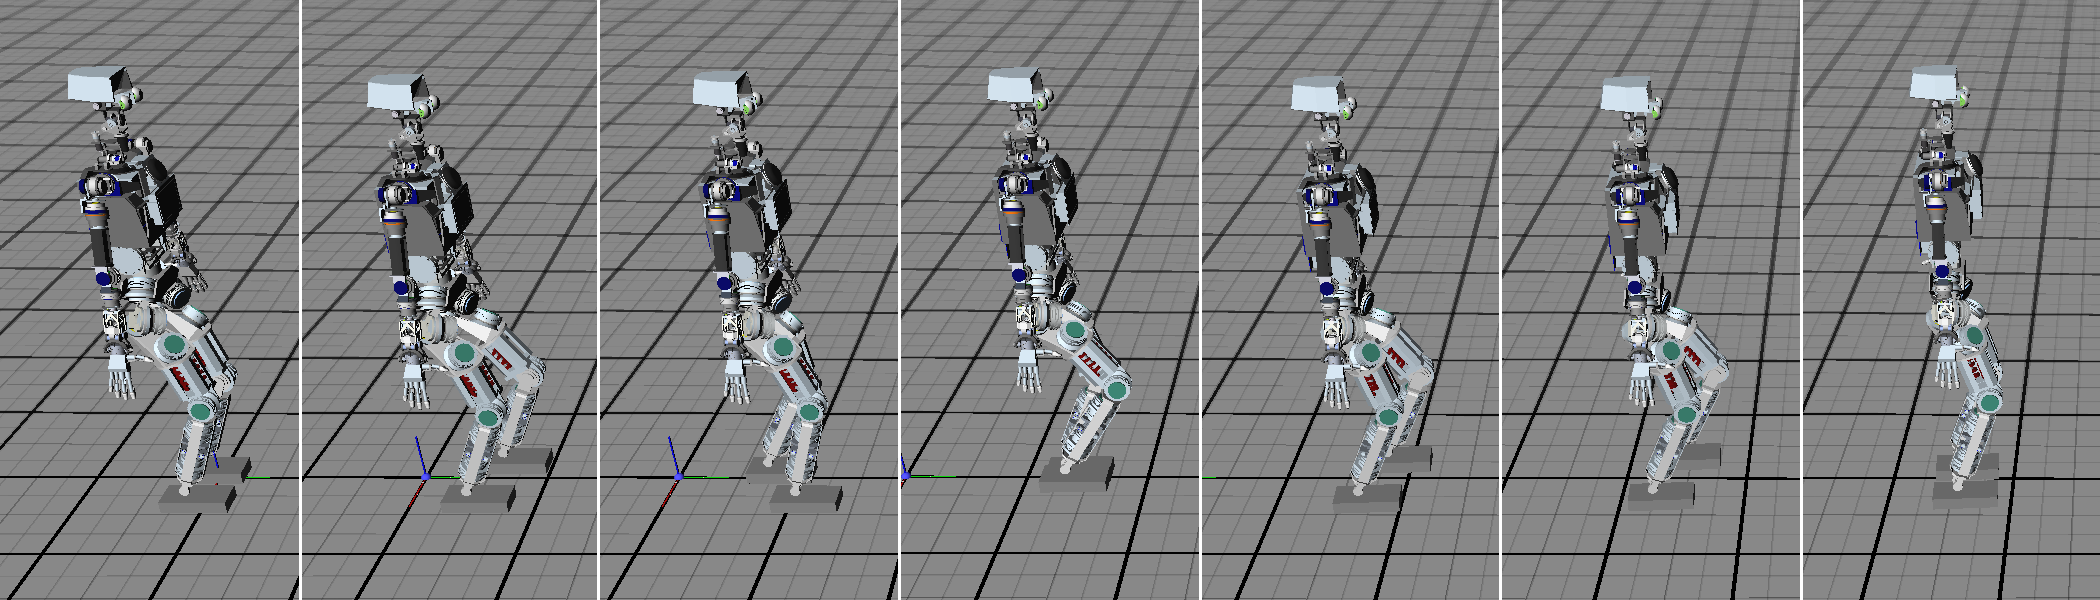
\includegraphics[width=\textwidth]{images/player_undisturbed_straight_thumbs.png}
\caption{Frames of undisturbed straight walking}
\label{img:player-undisturbed-straight-thumbs}
\end{figure*}

\begin{figure*}[hbt]
\vspace*{-1em}
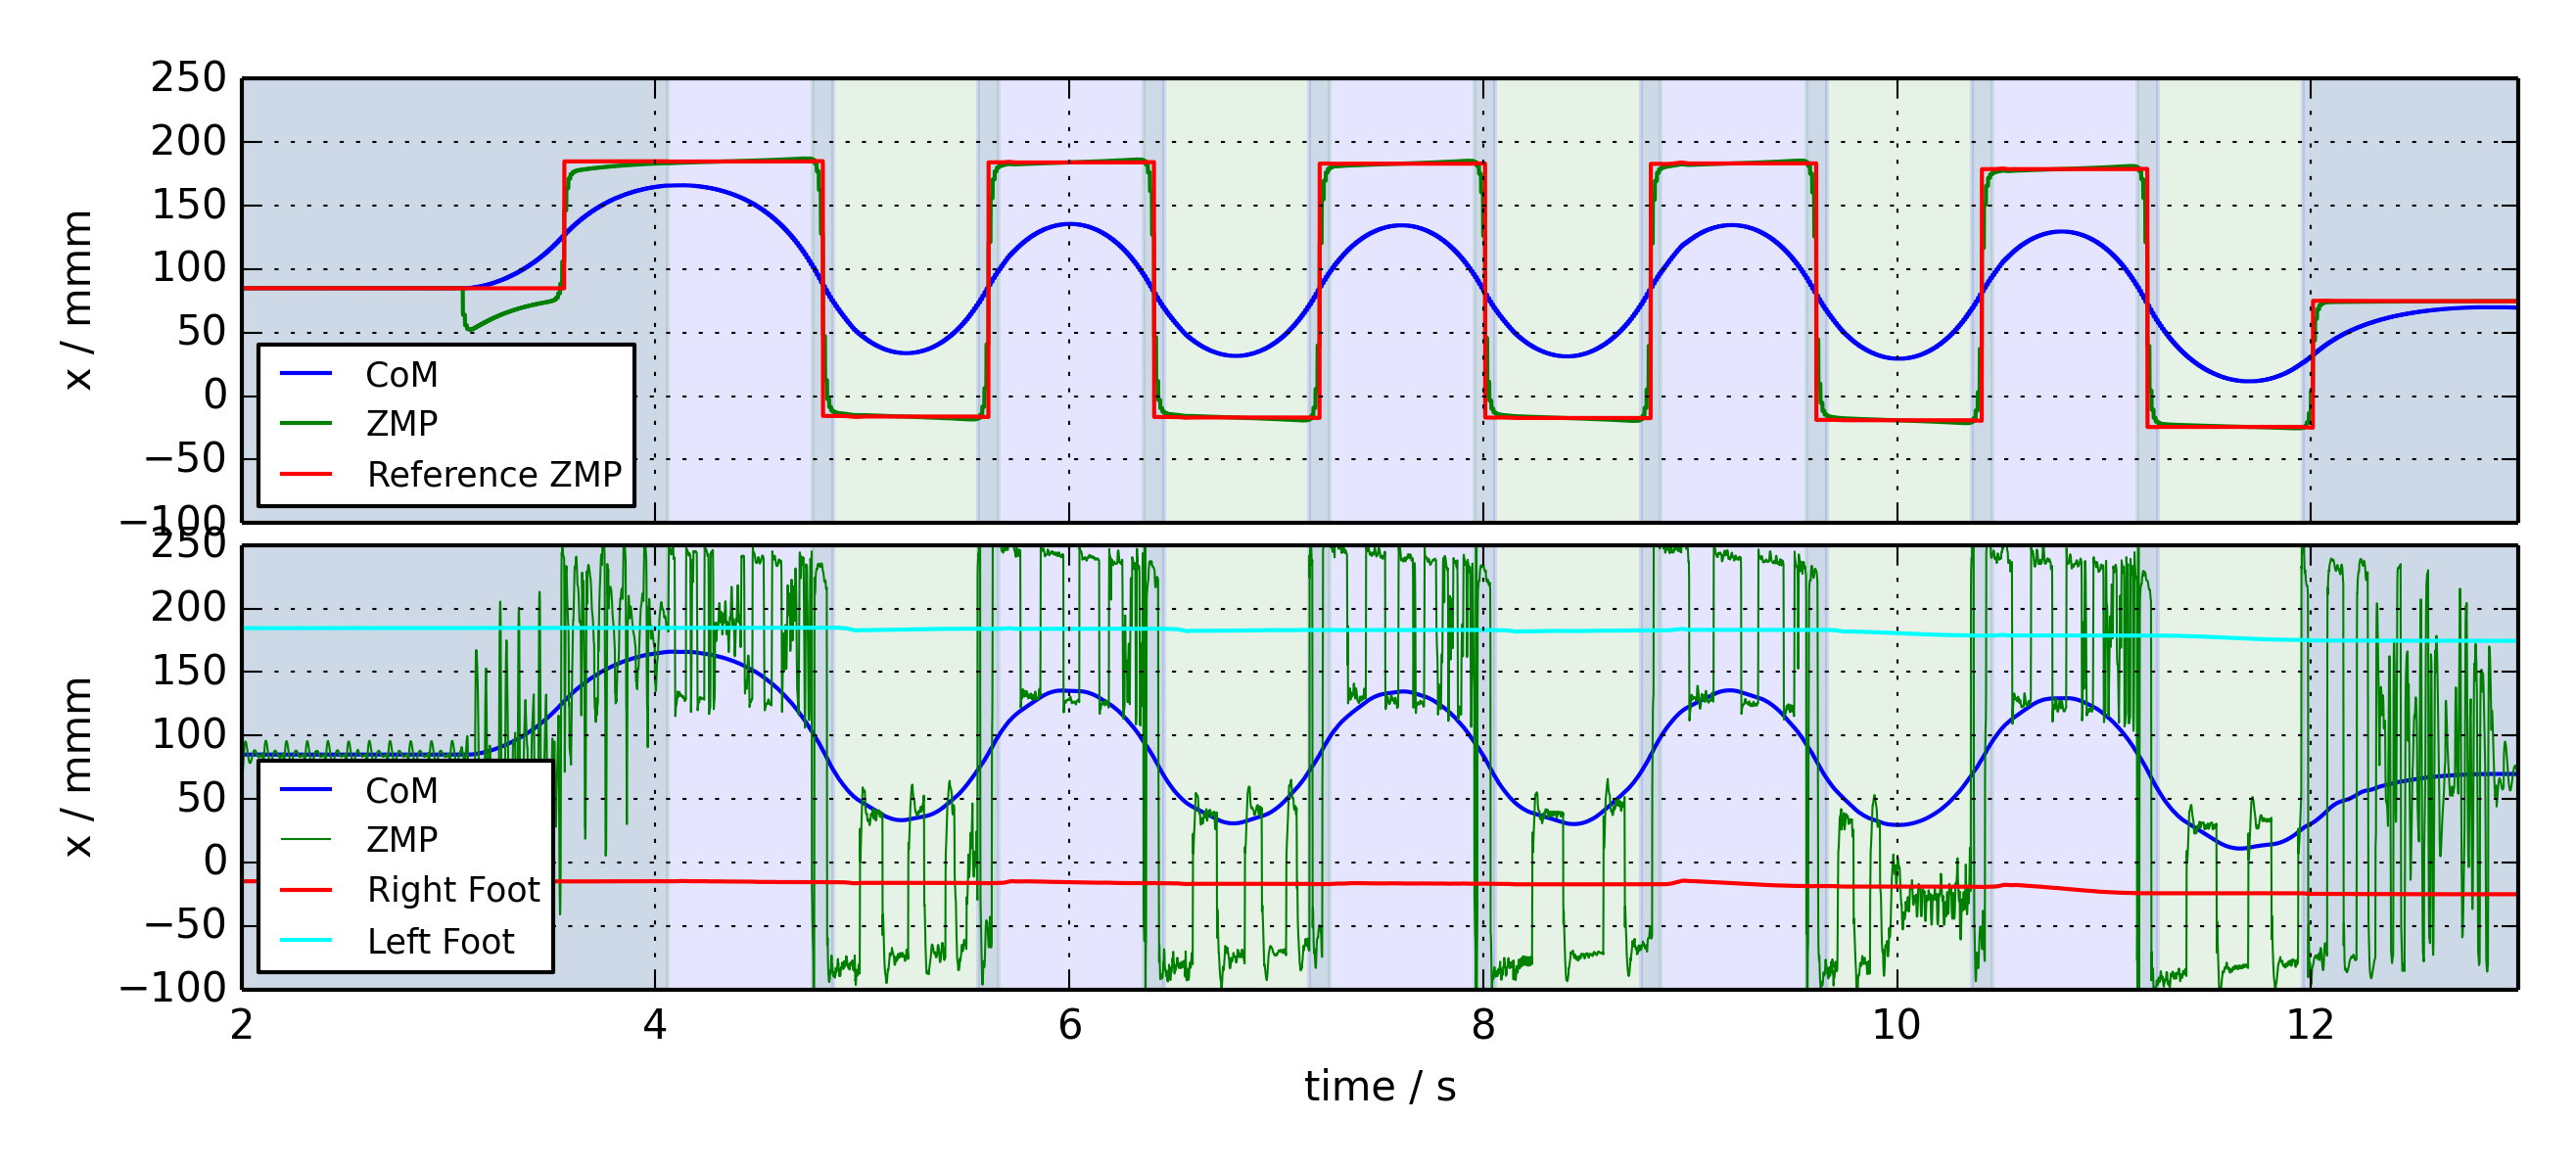
\includegraphics[width=\textwidth,resolution=300]{images/player_undisturbed_straight_x.png}
\caption{CoM and ZMP as specified by the pattern (top) and actual realized values (bottom).
All coordinates in the global reference frame.}
\label{img:player-undisturbed-straight-x}
\end{figure*}

\begin{figure*}[hbt]
\vspace*{-1em}
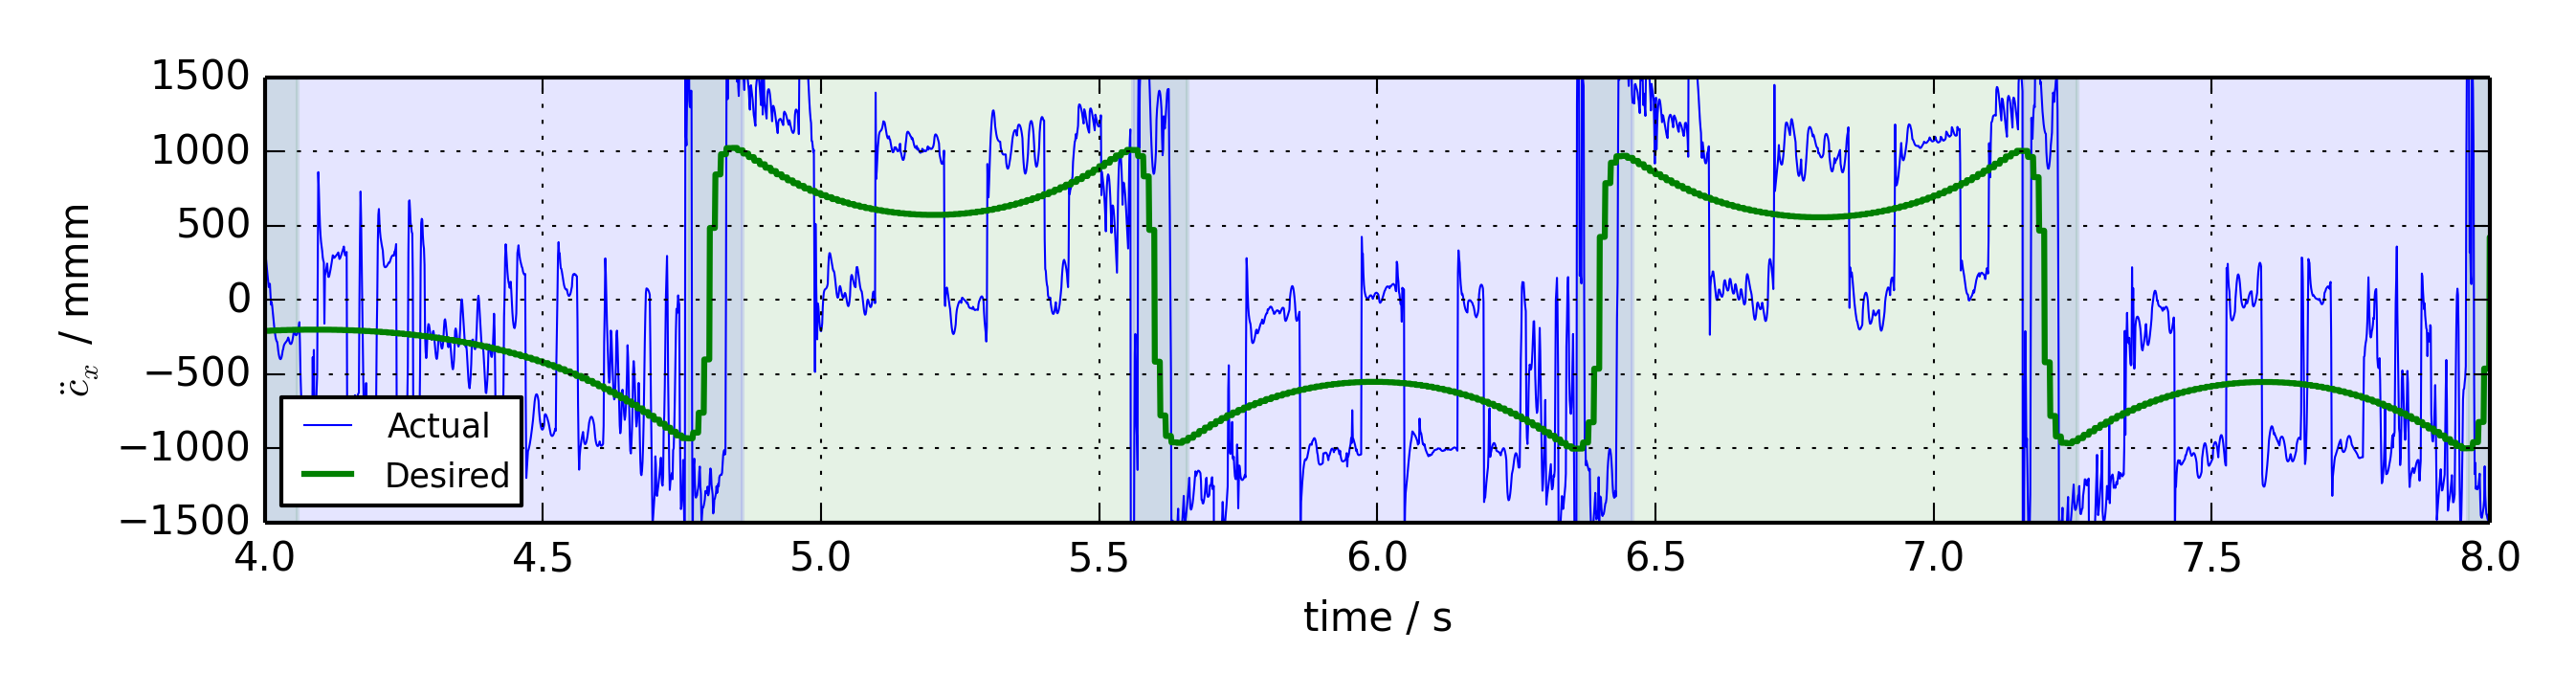
\includegraphics[width=\textwidth,resolution=300]{images/noisy_com_acc.png}
\caption{Acceleration of the CoM in $x$-direction.}
\label{img:noisy-com-acc}
\end{figure*}

\subsection{Walking in a circle}\label{walking-in-a-circle}

Figure \ref{img:player-undisturbed-circle-thumbs} shows the simulation
of walking in a circle. The robot walks in 12 steps in an arc of 180°
and 0.5 m radius. As you can see the desired 180° turn is not realized
completely. Due to the chest rotation following the tangent of the
circle, a torque around the yaw-axis is excerted on the foot. Recall
that during pattern generation we assumed that this torque is zero.
Since we do not correct this disturbance the trajectory deviates
significantly. \todo{read paper about yaw compensation} However stable
walking is still realized. See figure
\ref{img:player-undisturbed-circle}

\todo{image-series walking in a circle}

\begin{figure*}[hbt]
\vspace*{-1em}
% \includegraphics[width=\textwidth,resolution=300]{images/player_undisturbed_circle_thumbs.png}
\caption{\name{Armar4} walking in a half circle in 12 steps.}
\label{img:player-undisturbed-circle-thumbs}
\end{figure*}

\begin{figure}[hbt]
\vspace*{-1em}
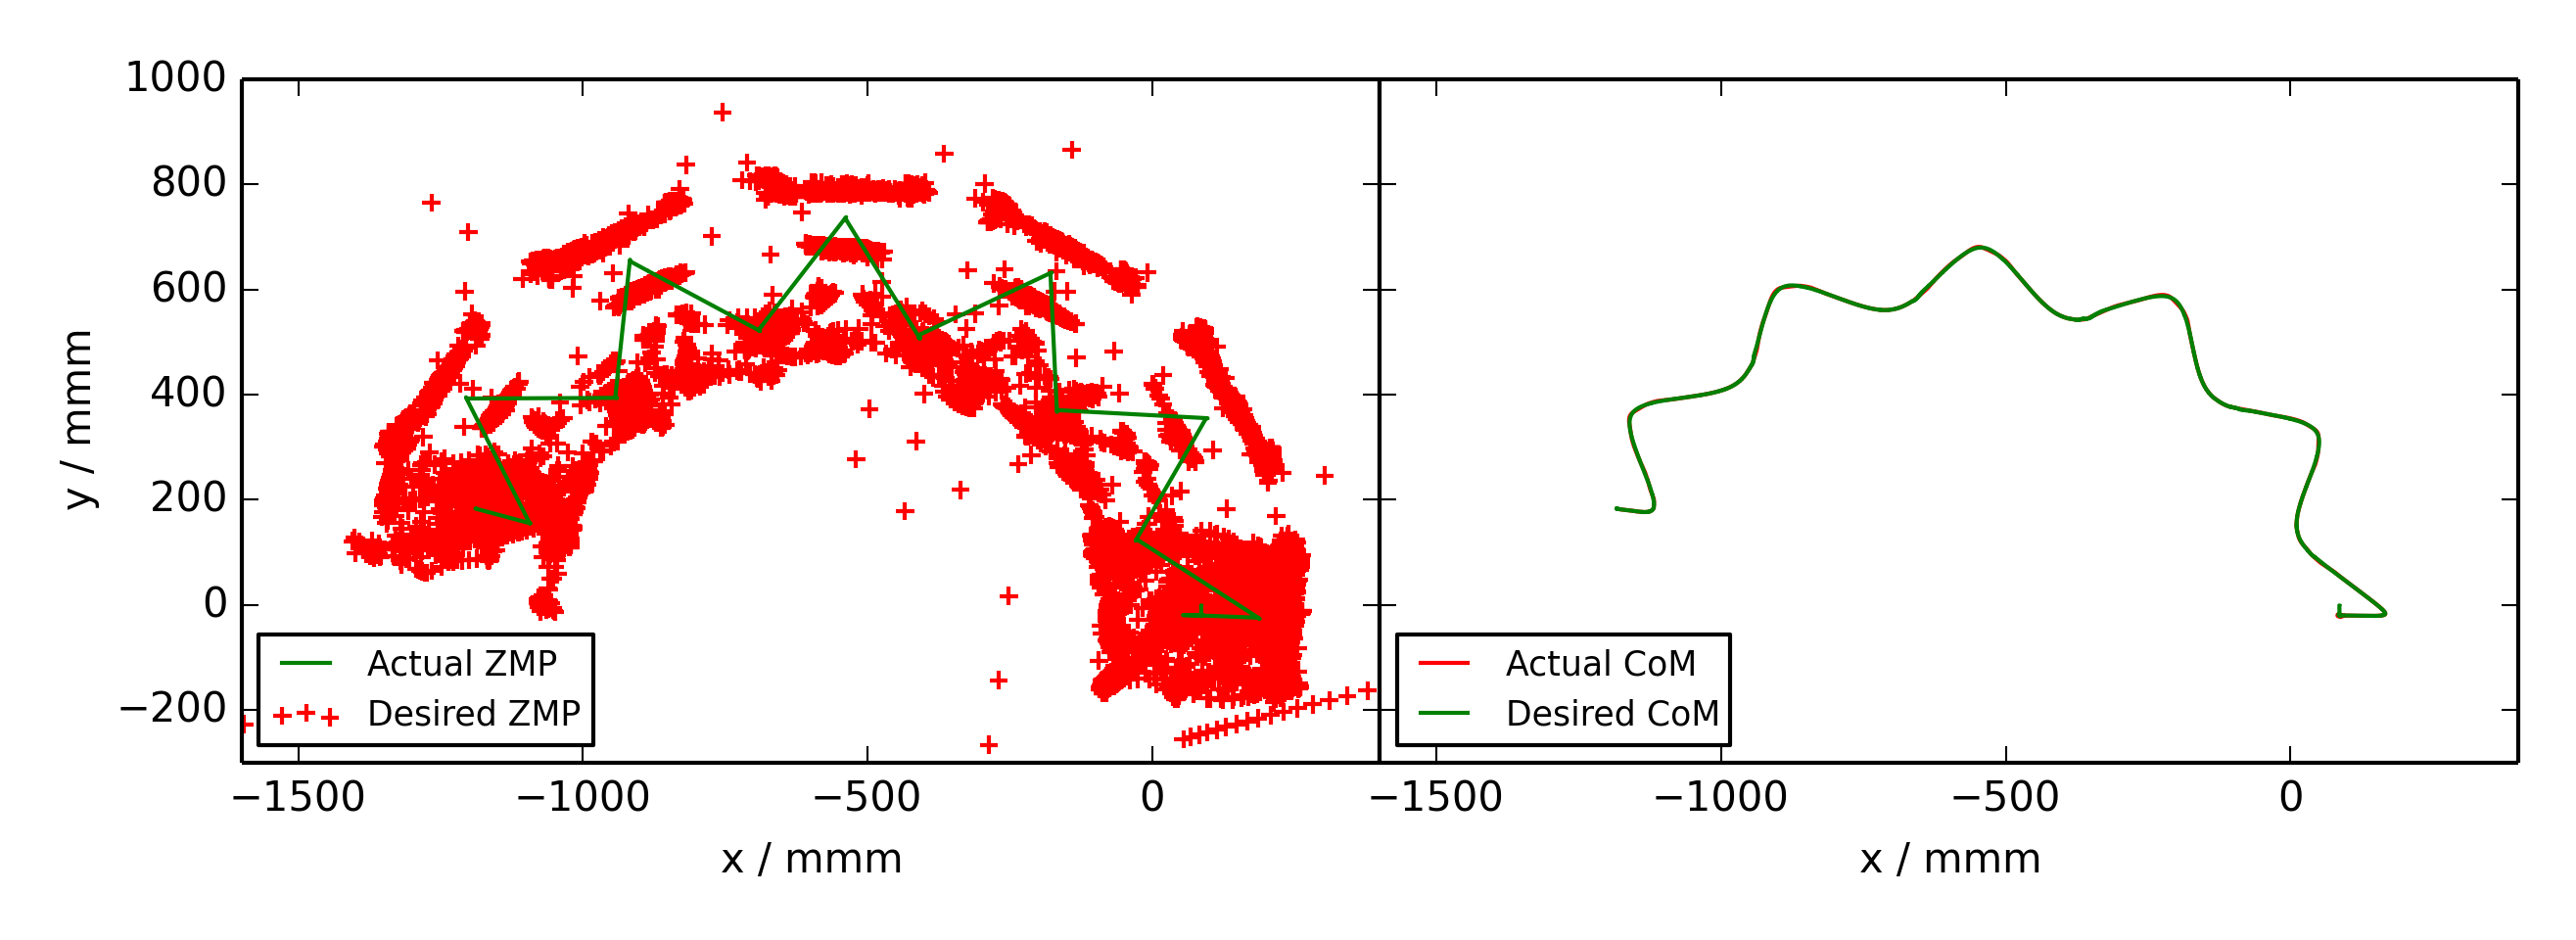
\includegraphics[width=\textwidth,resolution=300]{images/player_undisturbed_circle.png}
\caption{ZMP (left) and CoM (right) as specified by the pattern and the actually realized values.}
\label{img:player-undisturbed-circle}
\end{figure}

\section{Stabilized walking}\label{stabilized-walking}

In this section we present the results of using the alternative
stabilizer derived from the Kajita Stabilizer. As was the case with
unstabilized walking, a stable walking trajectory is realized. Smaller
disturbances can be corrected to remain stable.

\section{Undisturbed walking}\label{undisturbed-walking}

Figure \fixme{ref} and \fixme{ref} show the realized ZMP and CoM
trajectory of the same for walking straight and in a circle. As input
trajectories for the stabilizer the trajectorie tested in the previous
section are used.

The trajectory deviates a little more than it was the case for
unstabilized walking. This is somewhat expected, since the stabilizer
modifies the reference trajectory to ensure the constrains outlined in
\ref{section:alternative-approach}.

\todo{actual-zmp-straight} \todo{actual-zmp-circle}

\section{Disturbed walking}\label{disturbed-walking}

To test the performance of the stabilizer under disturbance, we used two
scenarios: A short push applied to the chest and slightly sloped ground.
The results are compared with the performance of the unstabilized
trajectory.

\subsection{Push to the chest}\label{push-to-the-chest}

To simulate a push, a ball with a radius of 11cm and weight of 450g
(FIFA football) is shoot from 2m distance at the chest.
\todo{force is meaningless as we don't know the units. Maybe print ball velocity on impact}
The point of impact is denoted as red lines.

\todo{actual-zmp-stabilized actual-zmp-unstabilized} \todo{image-series}

\chapter{Conclusions}\label{conclusions}

things to improve summary of work done and results

\chapter{TODO}\label{todo}

\listoftodos

\bibliographystyle{dinat} %-Deutsch

\bibliography{ba}

\end{document}
